\documentclass[11pt]{article}
\usepackage{graphicx}
\usepackage{caption}
\usepackage{subcaption}
\usepackage{hyperref}
\usepackage[a4paper, portrait, margin=1in]{geometry}

\usepackage{mathtools}
\DeclarePairedDelimiter{\ceil}{\lceil}{\rceil}

\begin{document}

\title{Advanced Systems Lab (Fall'16) -- Second
Milestone}

\author{Name: \emph{Aleksander Matusiak}\\Legi number: \emph{16-931-925}}

\date{
\vspace{4cm}
\textbf{Grading} \\
\begin{tabular}{|c|c|}
\hline  \textbf{Section} & \textbf{Points} \\ 
\hline  1 &  \\ 
\hline  2 &  \\ 
\hline  3 &  \\ 
\hline \hline Total & \\
\hline 
\end{tabular} 
}

\maketitle

\newpage

\section{Maximum Throughput}
\label{sec:max-throughput}

%Find the highest throughput of your system for 5 servers with no replication and a read-only workload configuration. What is the minimum number of threads and clients (rounded to multiple of 10) that together achieve this throughput? Explain why the system reaches its maximum throughput at these points and show how the performance changes around these configurations. Provide a detailed breakdown of the time spent in the middleware for each operation type.

\subsection{Hyphotesis}

The throughput, as we increase the number of clients, should be increasing, at least to the point where my middleware encounters problem. At first it will increase significantly, only to slow down later. However, as we could already see on the plot for baseline experiment in the milestone 1 the mean response time increased almost in a linear way and I predict similar behavior here (which is a consequence of the interactive response time law). This means that the maximal effective throughput will be probably achieved for not that big number of clients - for higher number of clients throughput will probably still increase slightly, but the response time would increase much faster. I predict that the saturation would be for number of clients from range 200 - 400.

The throughput, as we increase the number of threads in the thread pool, should also be increasing. However, creating more threads is associated with more overhead from operating system and might not improve the throughput as much as we would expect. I predict that using 20 - 40 threads will enable us to achieve the best performance.

% I predict that the bottleneck for the middleware would be the receiving of incoming client requests and putting them into an appropriate queue, since it is performed by only one thread, while every other operation can be executed by multiple threads in parallel. This means that at some points increasing the number of threads in the thread pool would not affect the throughput significantly - it will be limited by the bottleneck, which isn't affected by the increase of threads.


\subsection{General experimental setup}
Using memaslap in the read-only configuration means that before actual statistics are being displayed there is a phase where each memaslap clients sends only set requests in order to fill up the server with some keys, which it can later query. This phase was initially taking a very long time due to the default window size. Therefore, for all the experiments in this task I have decreased the window size for each memaslap client to 1k, which made initial phase with only set requests much shorter (lasting less than one minute). However, different servers still could finish initial phase much before others. Therefore, to be sure that during actual measurement all memaslap servers are sending only get requests, I have conducted the experiments with 1 minute warm-up and 1 minute cool-down phase.
% for 5 minutes and for calculating statistics I have used only the third minute. This means 2 minutes for warm up phase and 2 minutes for cool down phase, 
This time will include waiting with measurements for other servers to stop sending set requests. I have collected statistics every second. I have divided the interval of 3 minutes into 3 intervals, each 1 minute long. This means that for each configuration I have collected $3\cdot60$ numbers, from which I could calculate average, standard deviation and, when applicable, percentiles. Due to the limit of money I was able to use for this milestone (my subscription was renewed on 1st November), I couldn't afford a proper repetition of the experiment. Even though I was left with some funds near the end of the milestone, conducting repetition experiments not immediately after the original one, would not give any positive contribution for my experiments, since the results would differ significantly due to uncertainty of the Azure cloud. This means that I would have to repeat all the experiments from this part, as well as experiments for next chapters, which depend on the results of this experiment. This is why I have measured the behavior of the middleware for quite a long time (3 minutes), which enabled me to collect 3 results, one for every minute. 
I strongly believe that collecting 180 values for each configuration, as described above, provides statistical significance for my experiments.   

To avoid memcached misses I have increased the memory of each memcached server to 256\;MB.

\subsection{General plots description}
\label{sec:max-throughput-plots}

For every throughput plot I have indicated also standard deviation, which is based on $3\cdot60$ collected measurements. In order to make standard deviation visible for every line, I have shifted standard deviation right for each number of thread.

Every response time also includes lines for 25th and 90th percentile (no 50th percentile in order to improve readability of plots and response time in this experiment should be close to standard distribution). In order to make these lines more distinguishable, for every number of threads I have shifted the line up. I have to stress here, that these lines provide only a very rough approximation. This is the result of the following factors:
\begin{itemize}
\item Memaslap logs that enable us to count the appropriate percentile are produced only for the whole duration of the experiment (5 minutes). Therefore, these percentiles also include warm-up and cool-down phases. However collecting the data over a long period of time might have reduced inaccuracy connected with this factor. This is also another reason why I have decided to conduct long experiments rather then repeat short experiment a couple of times - the data for percentiles is more accurate.
\item The size of the ranges for which we know the number of requests with the value inside this range, is increasing twice by every step. This means, that we are unable to collect exactly the desired number of percentiles - the number of requests for some ranges is simply too large. I tried to use the best approximation and choose to plot actually the closest percentage that data produced by memaslap allows me to achieve.
\end{itemize}

\subsection{Overall experiment}
The purpose of this experiment was to gain a general understanding of the behavior of the system while varying the number of clients and threads significantly. It was conducted using the following scheme:
\medskip

{\small
\smallskip
\begin{tabular}{|c|c|}
\hline Number of servers & 5 \\ 
\hline Number of client machines & 5 \\ 
\hline Virtual clients / machine & 10 - 100 \\ 
\hline Step for virtual clients / machine & 10 \\ 
\hline Threads in the thread pool & 10 - 60 \\
\hline Step for threads in the thread pool & 10 \\
\hline Workload & Key 16B, Value 128B, Writes 0\% \\
\hline Middleware & No replication \\ 
\hline Runtime x repetitions & 5 min x 1 \\ 
\hline Warm-up phase & 1 min \\
\hline Cool-down phase & 1 min \\

\hline Log files & \parbox[t]{8cm}{overall\_1, overall\_2, overall\_3, overall\_4, overall\_5, \\ overall\_general} \\[3.4ex]
\hline 
\end{tabular} }
\medskip

Sampling rate in this experiment, as well as in all the experiments for this milestone, have stayed at the default level - 100 request.

I have combined the overall results from 3 partial results (one minute of the experiment). The variation between repetitions for average was quite small - values differed from average: for throughput at most 5.4\%, for response time - at most 2.3\%. However the variation for standard deviation was bigger - they differed from average standard deviation: for throughput - at most 34.5\%, for response time - 11.6\%. The bigger value here for throughput stems from the fact, that we are counting standard deviation of throughput for 60 values, and for the response time - from every request (it's done by memaslap). Therefore, standard deviation for response time more precisely corresponds to reality and therefore it varies less than this for throughput. All of these shows us that variation of data was huge, even between the experiments.


\begin{figure}
\centering
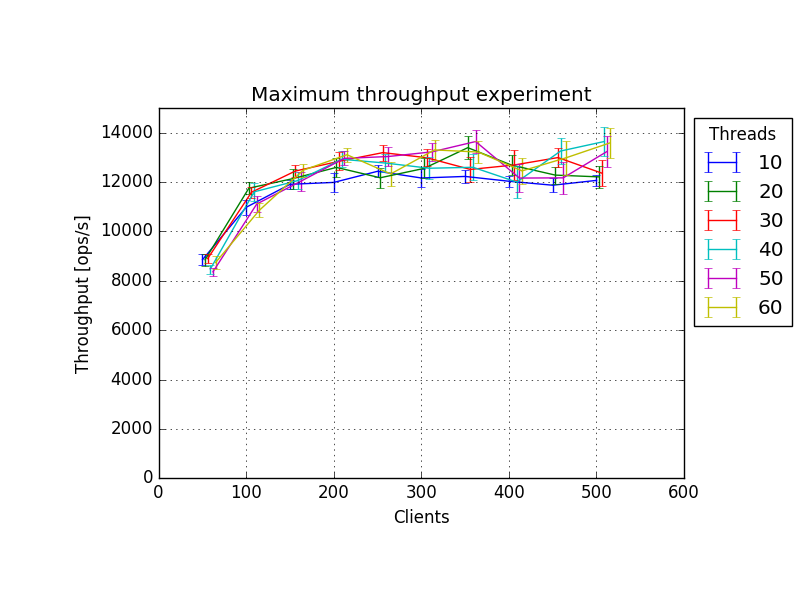
\includegraphics[width=0.95\linewidth]{plots/max_throughput_all_overall}
\caption{Plots for various number of threads in the overall experiment - throughput}
\label{fig:max-throughput-overall-throughput}
\end{figure}

\begin{figure}

\begin{subfigure}{\textwidth}
	\centering
	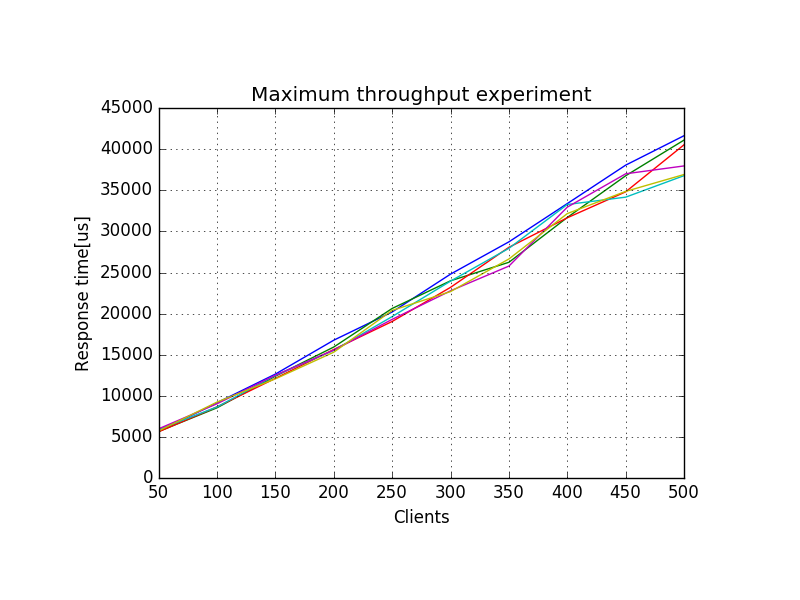
\includegraphics[width=0.95\linewidth]{plots/max_throughput-response_time_all_overall}
	\caption{Response time (with percentiles)}
\end{subfigure}
\begin{subfigure}{\textwidth}
	\centering
	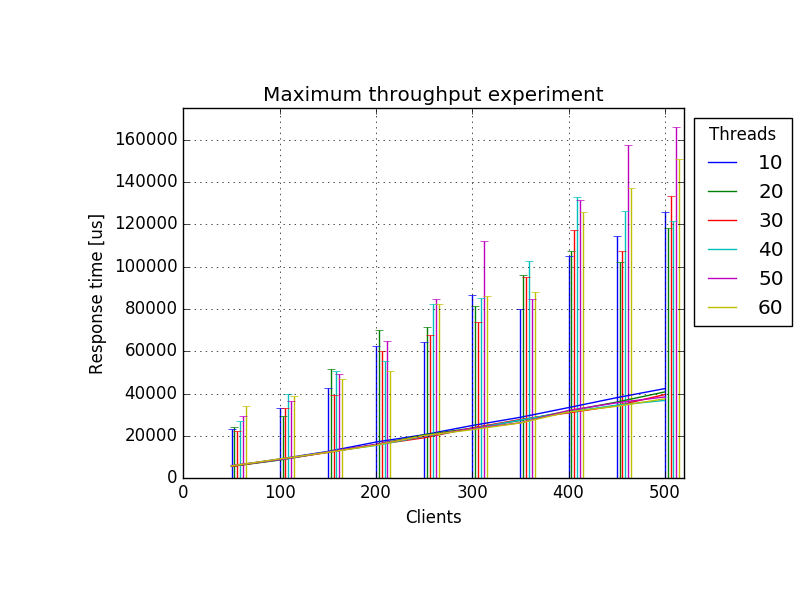
\includegraphics[width=0.95\linewidth]{plots/max_throughput-response_time_all_overall_std}
	\caption{Response time (with standard deviation)}
\end{subfigure}
\caption{Plots for various number of threads in the overall experiment}
\label{fig:max-throughput-overall-time}
\end{figure}

Results of this experiments are visible in the figure \ref{fig:max-throughput-overall-throughput} and \ref{fig:max-throughput-overall-time} (I have split response time with appropriate statistics into separate plots to improve readability).

As we can see from the plots, the throughput up to 500 clients is slightly growing. However, the response time is also growing in almost linear manner. This means that the maximal effective throughput should be achieved by clients in range around 150 - 250 clients. More precisely, the highest throughput for my experiment was achieved using 500 clients and 40 threads in the thread pool - it was equal to 13660 ops/s and it was corresponding to the mean response time equal to around 36790 us. If we look at the range 150-250 clients, the highest throughput was achieved for 250 clients and 30 threads - it was equal to 13171 ops/s and it was corresponding to mean response time equal to around 19099 us. This means that by limiting our analysis to range till 250 clients, we get highest throughout worse by around 3,6\%, but the response time is around 48,1\% lower (better). This means that we can indeed concentrate on the number of clients till 250, since the increase of the number of clients above it will maybe slightly increase throughput, but the response time will grow significantly.

\iffalse
The values that we got here correspond nicely to results predicted by the interactive law. Assuming time that clients waits before submitting next request equals approximately to 0, we have:
\medskip

\begin{tabular}{|c|c|c|c|}
\hline \bf{Clients} \# & \bf{Throughput [ops/s]} & \parbox[t]{4cm}{\bf{Response time [us]\\(measured)}} & \parbox[t]{4cm}{\bf{Response time [us] \\(interactive law)}} \\[3ex]
\hline 500 & 13660 & 36790 & 36603 \\
\hline 250 & 13171 & 19099 & 18981 \\
\hline
\end{tabular}
\medskip
\fi

It must also be pointed out here that number of threads does not make such a big difference as one could expect. We can clearly see in the plot that the middleware having 10 threads in each of the thread pool is performing noticeably worse then the middleware having more threads. We can still see that below 300 clients the middleware with the thread pool of size 20 is performing less effective than with other configurations. However, for bigger number of clients and size of the thread pool, difference in performance is not really significant. Therefore, as the optimal number of threads I have chosen 30 threads, since lower number of threads results in noticeably lower performance and higher number of threads does not make a significant difference. When we also take a look at the percentiles for the response time, we can see that the increase for 90th percentile for 10 threads is achieved for lower number of clients than for the rest of threads values. Also the increase for 25th percentile for 20 threads is achieved for the lower number of clients. This indicates that with these 2 values of threads in the thread pool our middleware performs worse than with higher number of threads.

There are two reasons why this is the case. Firstly, for more threads the bottleneck for the middleware shifts to the process of receiving incoming requests from the clients (see subsection \ref{sec:max-throughput-explanation}).  Secondly, this is caused by %This will be thoroughly analyzed in the subsection \ref{sec:time-breakdown}. What is more, the reason for not big effect of the number of threads might be 
the overhead from operating systems. Having more threads costs some system resources and since the virtual machine has only 8 cores, the threads might not be in reality performing task in parallel, but rather one after another. What is more, most of the time will be spend in the servers, not in the queue, which will be analyzed thoroughly in the subsection \ref{sec:time-breakdown}.

\subsection{Detailed experiment}

The purpose of this experiment was to find out the more precise number of clients that achieve maximum effective throughput. Based on the analysis from the previous section, I have used 30 threads in the thread pool for this experiment. It was conducted using the following scheme:
\medskip

{\small
\smallskip
\begin{tabular}{|c|c|}
\hline Number of servers & 5 \\ 
\hline Number of client machines & 5 \\ 
\hline Virtual clients / machine &  20 - 60 \\ 
\hline Step for virtual clients / machine & 2 \\
\hline Threads in the thread pool & 30 \\
\hline Workload & Key 16B, Value 128B, Writes 0\% \\
\hline Middleware & No replication \\ 
\hline Runtime x repetitions & 5 min x 1 \\ 
\hline Warm-up phase & 1 min \\
\hline Cool-down phase & 1 min \\
\hline Log files & \parbox[t]{9cm}{detailed\_1, detailed\_2, detailed\_3, detailed\_4, detailed\_5, \\ detailed\_general, max\_throughput\_detailed} \\[3.4ex]
\hline 
\end{tabular} }
\medskip

I have combined the overall results from 3 partial results (one minute of the experiment). The variation between repetitions for average was quite small - values differed from average: for throughput at most 2.6\%, for response time - at most 1.4\%. However the variation for standard deviation was bigger - they differed from average standard deviation: for throughput - at most 17.6\%, for response time - 5.5\%. Again, for throughput we get here a higher value. All these values, however, are lower than corresponding values from the overall experiment, because we have less measurements in this experiment.

\begin{figure}
\centering
\begin{subfigure}{.5\textwidth}
	\centering
	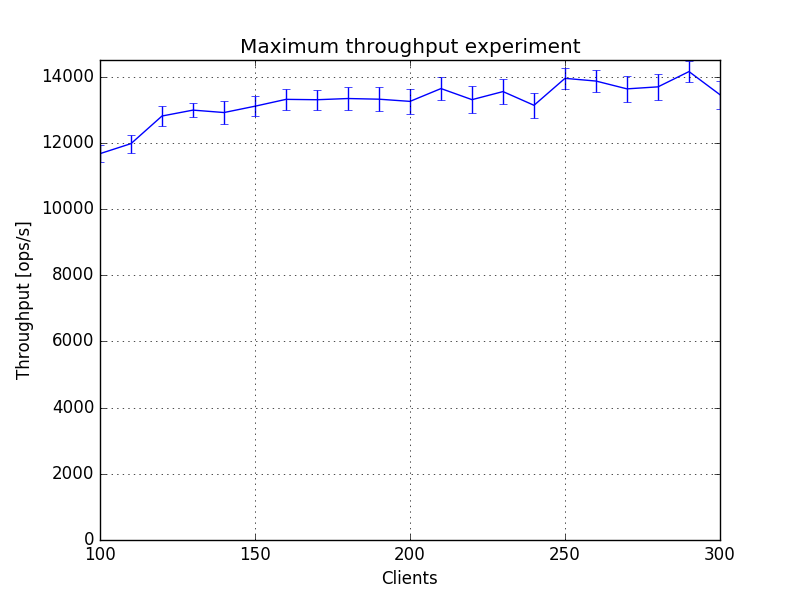
\includegraphics[width=\linewidth]{plots/max_throughput_all_detailed}
	\caption{Throughput}
\end{subfigure}%
\begin{subfigure}{.5\textwidth}
	\centering
	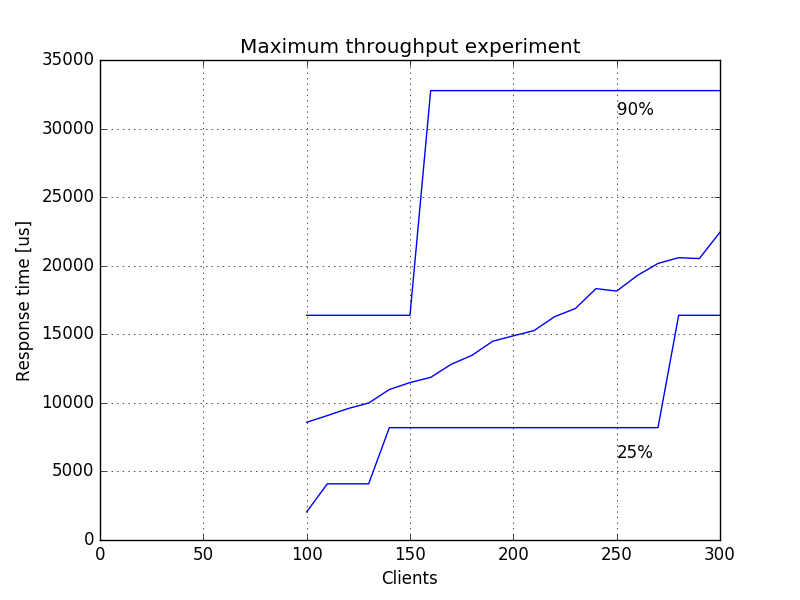
\includegraphics[width=\linewidth]{plots/max_throughput-response_time_all_detailed}
	\caption{Response time}
\end{subfigure}
\caption{Plots for various number of threads in the detailed experiment}
\label{fig:max-throughput-detailed}
\end{figure}

Results of this experiments are visible in the figure \ref{fig:max-throughput-detailed}. When we analyze this figure, there are 4 configurations that are to be considered when it comes to finding the maximal effective throughput. Data for these configurations is collected in the table below:

\medskip

\begin{tabular}{|c|c|c|c|}
\hline \bf{Clients \#} & \bf{Throughput [ops/s]} &\bf{Average response time [us]}  \\
\hline 160 & 13556 & 11858 \\
\hline 210 & 13812 & 15268 \\
\hline 250 & 13828 & 18149 \\
\hline 290 & 14201 & 20520 \\
\hline
\end{tabular}
\medskip

Although for these 4 configurations throughput is increasing as we increase number of clients, for the optimal number of clients I have chosen 210 clients. This is because till that point throughput increases significantly, after that it's still slightly increasing, but it's connected with much more increase in the response time. I have chosen 210 clients over 160 clients, since we can see from the plot that around 160 clients the throughput still have growing tendencies, while after 210 clients it's becoming more flat. What is more, 210 and 160 clients configurations have the same 25th and 90th percentile of the response time, so it's reasonable to choose one of them that has higher throughput.

To sum up, the maximal effective throughput is achieved for 210 clients and size of the thread pool equals 30. It is equal to around 13800 operations per second and corresponds to average response time equal to around 15250 us. Therefore, I will use 210 clients and 30 threads in the thread pool in later experiments.  

\subsection{Verification of the hypothesis}

As I have suspected, the number of clients for the maximal effective throughput was not that big and increasing number of clients further would only cause a slight increase in the throughput and a more significant increase in the mean response time. Further increasing of threads above 30 threads, which is inside the predicted range, does not contribute to the higher throughput.

\subsection{Breakdown of time spent in the middleware}
\label{sec:time-breakdown}

Since the purpose of this experiment was to analyze middleware under read-only workload, in this section I will provide breakdown of time spent in the middleware for get operations.
\medskip

In the whole report, whenever I mention queue time, I mean time spent by the requests in the queue, which is a component used in the middleware and described in the architecture description in the report for milestone 1. When I use servers time, I mean time for a given request from the moment the first forwarded request is sent to the servers till the last response is received. Therefore, this time includes sending the forwarded requests, time spent by the requests in the network and in the server, time spent by the responses in the middleware waiting to be processed, as well as processing these responses.
\medskip

\begin{tabular}{|c|c|c|c|c|c|}
\hline \bf{Time spent ...} & \bf{Avg. [us]} & \parbox[t]{1.9cm}{\bf{Std.\\dev. [us]}} & \parbox[t]{2.6cm}{\bf{Coefficient of \\variation}} & \parbox[t]{1.7cm}{\bf{25th \\per. [us]}} & \parbox[t]{1.7cm}{\bf{90th \\per. [us]}} \\[3ex]
\hline in the middleware & 6723 & 12213 & 1.76 & 801 & 12997 \\
\hline in the queue & 2557 & 7192 & 2.69 & 23 & 7952\\
\hline in the server & 4119 & 9329 & 2.22 & 550 & 9689\\
\hline \parbox[t]{3cm}{in the queue\\and the server} & 6676 & - & - & -&-\\[3ex]
\hline \parbox[t]{3cm}{being actively\\processed} & 47 & - & - & -&-\\
\hline
\end{tabular}
\medskip

\begin{figure}
\centering
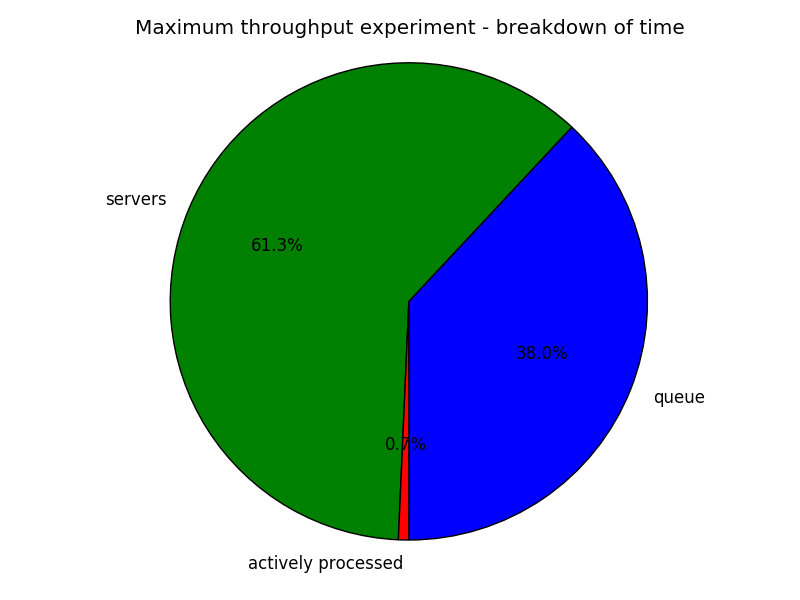
\includegraphics[width=0.5\linewidth]{plots/max_throughput-breakdown}
\caption{Breakdown of time spent in the middleware}
\label{fig:max-throughput-breakdown}
\end{figure}

As we can see from the above table and from the figure \ref{fig:max-throughput-breakdown}, most of the time (around 61\%) is spent by the requests in servers. Time spent in the queue is less significant (around 38\%). This is because we have chosen optimal number of threads to achieve the best performance. With 30 threads in the single thread pool (for each server), so in total with 150 threads processing get requests, we can process requests from 210 clients effectively. However, we must remember that the processor on the virtual machine on which the middleware server was running, has only 8 cores. Therefore, time waiting in the queue is not negligible and influences the total time spent in the middleware. But we can notice that 25th percentile for the queue is really low, which means that some requests spend almost no time in the queue.

It must be pointed out that the coefficient of variation for time spent in the queue is high, also comparing to time spent in the servers and total time in the middleware. This is because time spent in the queue depends also on other factors. If we have some disturbance in the network, threads processing get requests will have to wait longer for response from the server and therefore will not be able to take next requests of out the queue (getter threads are synchronous). What is more, if there is a disturbance in the network from client to the middleware server, workers might be idle, whereas when later huge number of requests come, they will not be able to process them effectively. This means that time spent in the queue depends significantly on other factors, which explains why it can vary noticeably.

\subsection{Explanation why the system reaches its maximum throughput at these points}
\label{sec:max-throughput-explanation}

As mentioned above, the reason why we cannot get much higher throughput when increasing the number of clients and threads is because the bottleneck of the system shifts to handling incoming requests. We could see from the breakdown analysis that time spent in the queue was relatively low compared to the time spent in the middleware. What is more, we know that memcached servers were not saturated - they had around 42 clients each, which, as we know from the milestone 1, is far from the saturation point of these servers (they became saturated for 96 clients). Furthermore, increasing number of threads did not increase the performance. These all factors indicate that it indeed is handling incoming threads that becomes the bottleneck of the system as we increase the number of clients and with reasonable number of threads in the thread pool. This can be also well explained in terms of the design of my middleware. There is only one thread handling incoming connections, parsing them, hashing the key and placing requests in the queue. Although this thread does not have to wait for responses from server, it still must process all the requests. Having many threads in the thread pool can improve performance of processing requests already in the middleware, but it may only affect negatively the thread accepting incoming requests. With many threads (for optimal configuration we have them in total 156), one thread handling incoming requests might not get as much resources as it requires. We have not assigned one core to this thread that can only execute this thread, but rather operating systems has to choose when this thread is performed. Therefore, this thread becomes the bottleneck of the system. 


\clearpage

%-----------------------------------------------------------

\section{Effect of Replication}
\label{sec:replication}

\iffalse
Explore how the behavior of your system changes for a 5\%-write workload with S=3,5 and 7 server backends and the following three replication factors:
\begin{itemize} 
\item Write to $1$ (no replication) 
\item Write to $\ceil{\frac{S}{2}}$ (half) 
\item Write to all 
\end{itemize}

Answer at least the following questions: Are \texttt{get} and \texttt{set} requests impacted the same way by different setups? If yes/no, why? Which operations become more expensive inside the middleware as the configuration changes? How does the scalability of your system compare to that of an ideal implementation? Provide the graphs and tables necessary to support your claims.
\fi

\subsection{Hypothesis}
\label{sec:replication-hyphotesis}

As we increase the replication factor (number of servers to which we send each set request), the performance of the middleware should decrease. This is quite obvious - we have to send more set requests to servers and then receive and process all the replies. What is more, memcached servers will have more write requests, which might also lower the performance of the whole system. With higher replication factor we should also have higher variation of the data, since we will be more prone to network latencies. Behavior described in this paragraph should be mostly visible for set requests, but since they consist of 5\% of the requests, it shall also affect overall performance. I predict that the replication should not influence significantly the time spent in the middleware for get requests since replication configuration changes change only how set workers perform their tasks.

I also expect the performance to increase when we go from 3 to 5 servers and decrease as we go from 5 to 7 servers. This is because we chose number of threads optimal for 5 servers, but we also get more threads overhead as we increase the number of servers.

\subsection{Experimental setup}

The experiment was conducted using the following scheme:

{\small
\smallskip
\begin{tabular}{|c|c|}
\hline Number of servers & 3 - 7 \\ 
\hline Step for number of servers & 2 \\
\hline Number of client machines & 3 \\ 
\hline Virtual clients / machine &  70 \\ 
\hline Threads in the thread pool & 30 \\
\hline Workload & Key 16B, Value 128B, Writes 5\% \\
\hline Middleware & Replication: none, half, all \\ 
\hline Runtime x repetitions & 3 min x 3 \\
\hline Warm-up phase & 1 min \\
\hline Cool-down phase & 1 min \\
\hline Log files & \parbox[t]{10cm}{replication\_1, replication\_2, replication\_3, \\replication\_general, replication\_middleware} \\[3.4ex]
\hline 
\end{tabular} }
\medskip

For window size I have stayed with 1k, in order to be consistent with the previous experiment (although it shouldn't change the performance)

I have combined the results from 3 repetitions. The variation between repetitions for average was small - values differed from average at most 2.1\%. However the variation for standard deviation was bigger - they differed from average standard deviation at most 13.1\%.  This shows that the overall variation of data was huge, even between the experiments.

\subsection{General plots description}
For throughput plots presented in this section and section \ref{sec:writes} I have indicated also standard deviation. For response times and time spent in the middleware (both in this and the next section) I have indicated standard deviation, as well as 25th, 50th and 90th percentile. Standard deviation is represented as a classic error bar, whereas 25th percentile is marked with white cross, 50th - yellow one, 90th - black one. It is worth mentioning here that although percentiles calculated on the memaslap logs provide very rough approximation (see \ref{sec:max-throughput-plots}), percentiles calculated for middleware times are more precise. For middleware we have collected more measurements and could calculate this percentiles ourselves (not really on bucket's approximation from memaslap).

In this section, as well as in the next one, the abbreviation $R$ can be used to refer to the replication factor.

\subsection{Overall performance}
\label{sec:replication-overall}

\begin{figure}
\centering
\begin{subfigure}{.5\textwidth}
	\centering
	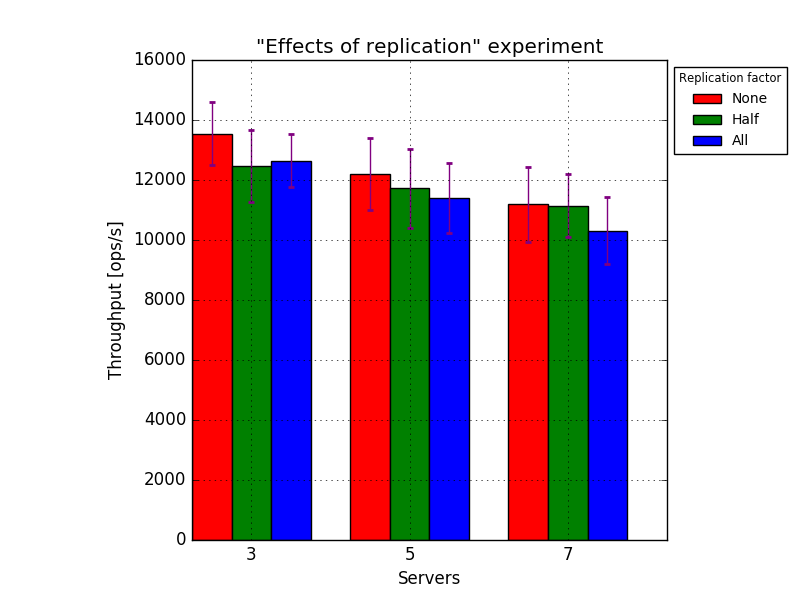
\includegraphics[width=\linewidth]{plots/replication}
	\caption{Throughput}
	\label{fig:replication-throughput}
\end{subfigure}%
\begin{subfigure}{.5\textwidth}
	\centering
	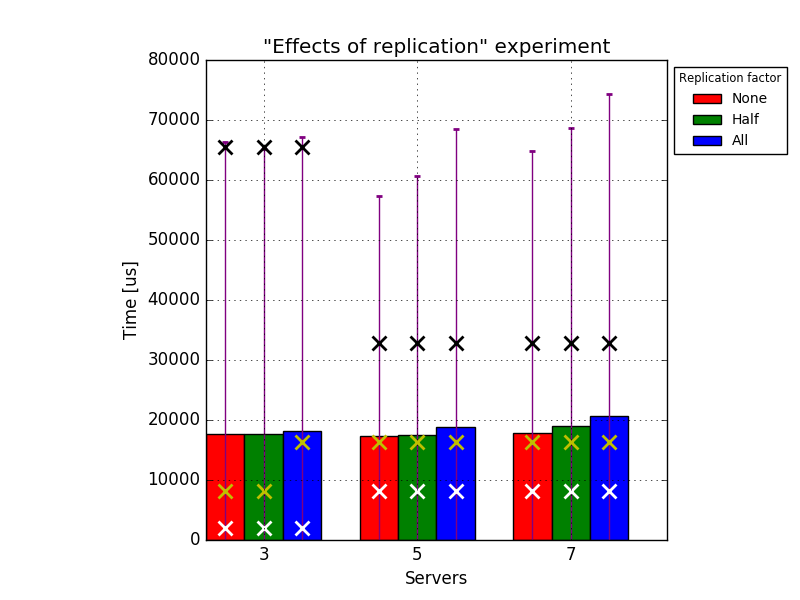
\includegraphics[width=\linewidth]{plots/replication-response_time}
	\caption{Response time}
	\label{fig:replication-reponse-time}
\end{subfigure}
\caption{Overall performance for the replication experiment}
\label{fig:replication-overall}
\end{figure}

As we can see from figure \ref{fig:replication-overall}, performance of the system (measured as the throughput and response time) for 5 and 7 servers is decreasing as we increase the replication factor. For 3 servers we can also notice that as we increase replication factor from half to all, the performance decreases, but when we increase the replication factor from none to half we can notice a slight increase of the performance. However, the difference between these values is within statistical error.

The performance of the middleware as we increase the replication factor was predicted properly in the section \ref{sec:replication-hyphotesis}. However, we can't notice the change in standard deviation of the throughput as we increase replication factor. This might be because we measure throughput every second, so although we can get differences in performance within one second, they are smoothen out when we take the measurement from the whole second.
%The variation of data will be further analyzed in section \ref{sec:replication-set}, where we can get more accurate data as far as distribution of data is concerned.
%lso (for every replication factor). As we go from 3 to 7 servers we notice decrease in the performance (throughput) of 17\%, 11\% and 18\% for replication factor: none, half and all respectively. 

From the plot we can also see a slight increase in the performance when we increase the servers from 3 to 5 for replication factors none and half. This is because get requests for 5 servers spend much less time in the queue than for 3 servers. This behavior will be explained in the section \ref{sec:replication-get}. For other configurations (replication to all and changing from 5 to 7 servers) we see that the performance decreases as we increase the number of servers . With more servers we create more threads, which causes more overhead to our middleware. With only 8 cores available on the virtual machines, higher number of threads might cause threads fighting over processor resources, which leads to reduced performance. Although load for each server is lower with higher number of servers, the bottleneck of the whole system is middleware and overhead on the middleware causes lower performance.

\subsection{Scalability of the system}
Following the analysis presented in the section \ref{sec:replication-overall}, we can conclude that our system does not provide good scalability. As we increase number of servers in the ideal system, the performance of the system should increase, since there would be less load on each server. However, the experimental result show opposite behavior - as we increase the number of servers (from 5 to 7), performance decreases. This enables us to conclude that memcached servers are not saturated and it is our middleware that is the bottleneck of the system. With more overhead on the middleware connected with more servers, we get noticeable worse performance.

What is more, the ideal scalability would also mean that increasing the replication factor should not influence the performance significantly. In the ideal world every request to the servers would take the same time and increasing sent requests would only cause our middleware to perform a little more work per request (since we have 5\% of writes requests, memcached servers wouldn't notice much change in the incoming requests). Comparing to time spent in the network and in the queue, it wouldn't affect overall performance much. However, our middleware almost always decreases in performance as we increase the replication factor. This is because of the increasing time spent in the servers for set requests and it will be analyzed in the section \ref{sec:replication-set}.

\subsection{Get requests}
\label{sec:replication-get}

\begin{figure}
\centering
\begin{subfigure}{.5\textwidth}
	\centering
	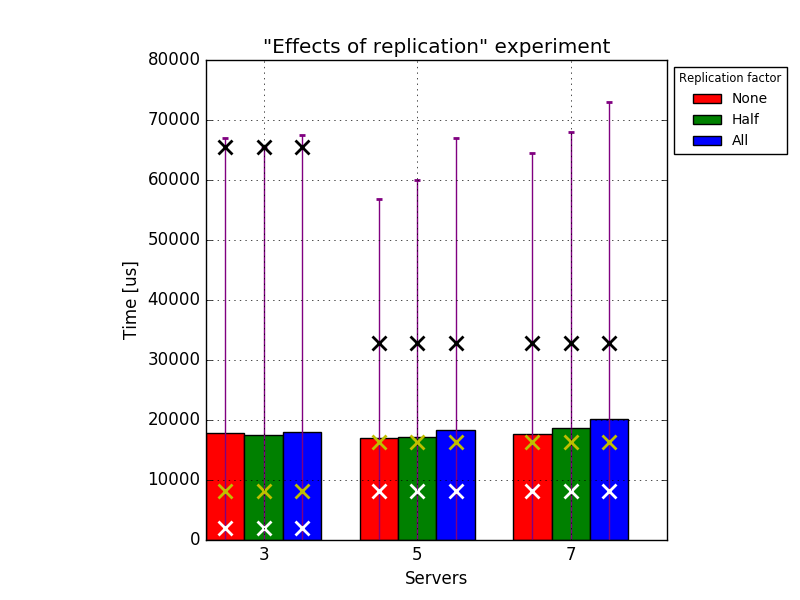
\includegraphics[width=\linewidth]{plots/replication-response_time-get}
	\caption{Response time}
	\label{fig:replication-response-time-get}
\end{subfigure}%
\begin{subfigure}{.5\textwidth}
	\centering
	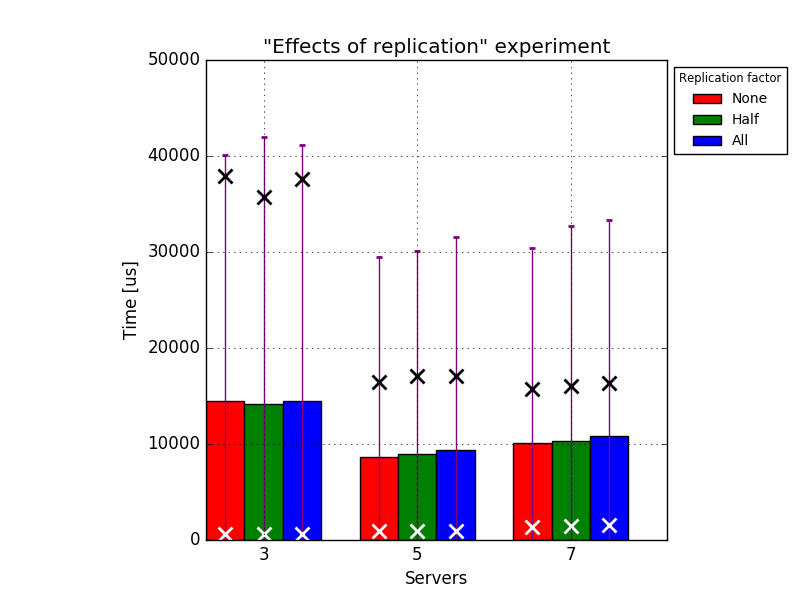
\includegraphics[width=\linewidth]{plots/replication-get}
	\caption{Total time in the middleware}
	\label{fig:replication-get-middleware}
\end{subfigure}

\caption{Measured times for get requests}
\label{fig:replication-get}
\end{figure}

We can see from the figure \ref{fig:replication-get} that get requests are not much affected by changing the replication factor. Differences between different replication factors are negligible, taking into the account how big is the standard deviation. This is because changing replication factor does not change the work that get workers have to do. There might be some additional load on the middleware connected with increased replication factor and also probably higher network traffic (more set requests), but as the plot shows, it does not matter that much for get requests. From figures \ref{fig:replication-get-queue} and \ref{fig:replication-get-servers} we also cannot see any significant difference in the time spent by the request for different replication factors.

\begin{figure}
\centering
\begin{subfigure}{.5\textwidth}
	\centering
	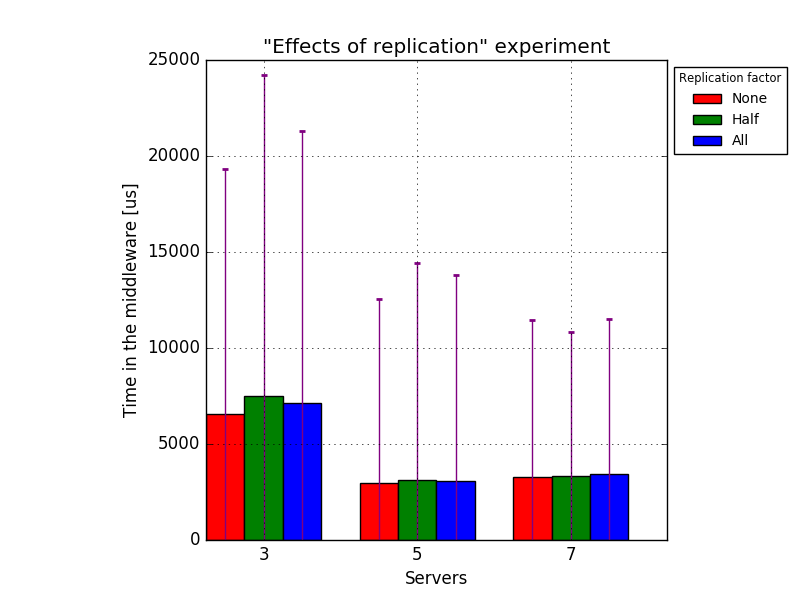
\includegraphics[width=\linewidth]{plots/replication-get-queue}
	\caption{Time in the queue}
	\label{fig:replication-get-queue}
\end{subfigure}%
\begin{subfigure}{.5\textwidth}
	\centering
	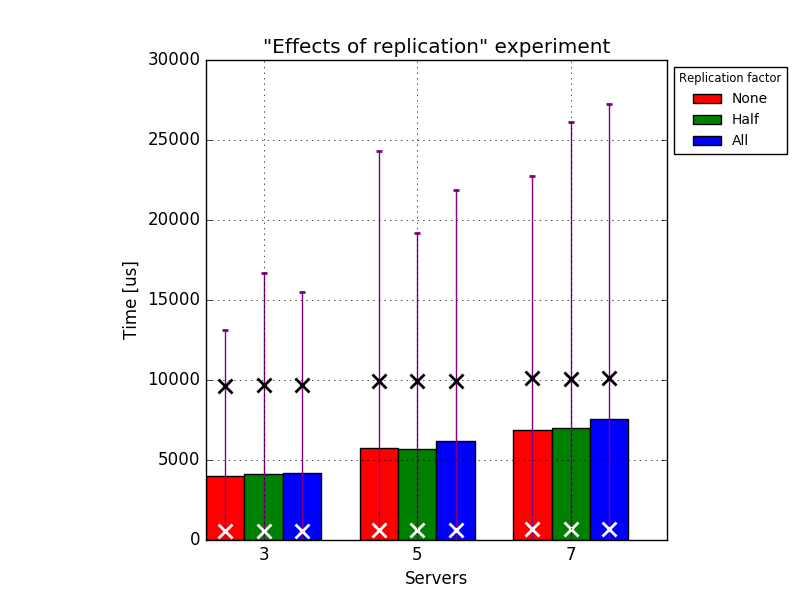
\includegraphics[width=\linewidth]{plots/replication-get-servers}
	\caption{Time in the servers}
	\label{fig:replication-get-servers}
\end{subfigure}
\caption{Breakdown of time spent in the middleware for get requests}
\label{fig:replication-get-breakdown}
\end{figure}

As we increase the number of servers from 3 to 5, we can see from the figure \ref{fig:replication-get} that the time spent in the middleware decreases. This can be explained by the decrease of time spent in the queue. However, we don't see any significant difference when it comes to the response time measured by memaslap clients. This is because with enough threads to process get requests, it is handling incoming requests that becomes the bottleneck of the system. The time spent by the request waiting for being handled by the accepting threads is not measured and we can only reason about it by comparing response times from memaslap clients and time spent in the middleware. This result is consistent with the section \ref{sec:max-throughput-explanation}, where we concluded that we cannot increase the performance because of the handling incoming requests being the bottleneck. What is more, with higher number of threads, one thread that processes incoming requests gets less processor resources and its performance can also decrease. So although we can notice time spent in the middleware descreasing, overall performance does not change much. 

Looking at the figure \ref{fig:replication-get-queue} we can see a significant decreasein the time spent in the queue as we increase number of servers from 3 to 5 - by around 57\%. This is because for 3 threads we do not have enough threads per request in the queue to allow to process threads from the queue efficiently. For 3 servers we have 70 requests and 30 threads per queue, which results in $2\frac{1}{3}$ requests per thread. For 5 servers: 45 requests and 30 threads, which corresponds to $1\frac{1}{2}$ requests per thread. This means that elements can be taken out of the quickly for 5 servers, because each server has lower number of requests it has to process. However, when we increase number of servers from 5 to 7 we do not see a significant difference in this value. This means that decreasing number of requests per one queue would not further affect the time spent in the queue. This might be because even while having better (smaller) requests per thread ratio, the overhead of operating systems with more threads will increase, therefore preventing the middleware to have better inside performance.

%It is worth noticing here that his result is consistent with my results of experiments described in the section \ref{sec:max-throughput}. Increasing number of servers here decreases the ratio of requests per thread (for a given queue), while increasing number of threads (with constant number of requests) also decreased this ratio. In the section \ref{sec:max-throughput} we have concluded that number of threads in the thread pool equal to 30 is optimal. We used the same number of threads in this experiment. Therefore, increasing number of servers from 3 to 5 should correspond to increasing number of threads to 30 in the maximal throughput experiment, while increasing number of servers from 5 to 7 corresponds to increasing number of threads from 30 upward, which did not yield a noticeable difference.

When we look at the figure \ref{fig:replication-get-servers} we can see that increasing number of servers increases the time spent in the servers. This is because of more overhead from the side of the middleware - getter threads are not longer that effective, because of the operating system overhead (e.g. overhead of changing context) connected with more threads. It takes longer to send and receive the message with more servers (which is counted as server time). What is more, with many threads and only 8 cores, for some of the responses coming back from the server it might be not be able to process them immediately (processors cores will have some other threads running), which will cause increase in the server time. There is also one more factor that causes this. Mainly, when we look at the percentiles in the figure \ref{fig:replication-get-servers}, they are very similar. This, alongside with increase of the average, means that with more servers we have more requests that are processed way longer than the rest. This is basically connected with the network instability, which increases as we are using more servers. 

All the data presented in this section comes with high standard deviation. From figure \ref{fig:replication-get} we can see, however, that although response time and time in the middleware do not change significantly as we increase the replication factor, the increase in the standard deviation is more significant. What is more, as we go from 3 to 5 servers, we can notice decrease in the 90th percentile for the response time and standard deviation (for replication factor: none and half). This is connected with decrease in the time spent in the middleware and response times depending mostly on one component (accepting requests), which makes data less varied. When it comes to percentiles, we can notice that for the queue time 25th and 50th percentiles are really small. This means that often requests spend very little time in the queue, which corresponds to the situation where requests are almost immediately processed by a getter thread. This is possible because we use a reasonable number of threads in the thread pool. What is more, queue time depends strongly on overall performance of the system and has higher variation of data.

\subsection{Set requests}
\label{sec:replication-set}

\begin{figure}
\centering
\begin{subfigure}{.5\textwidth}
	\centering
	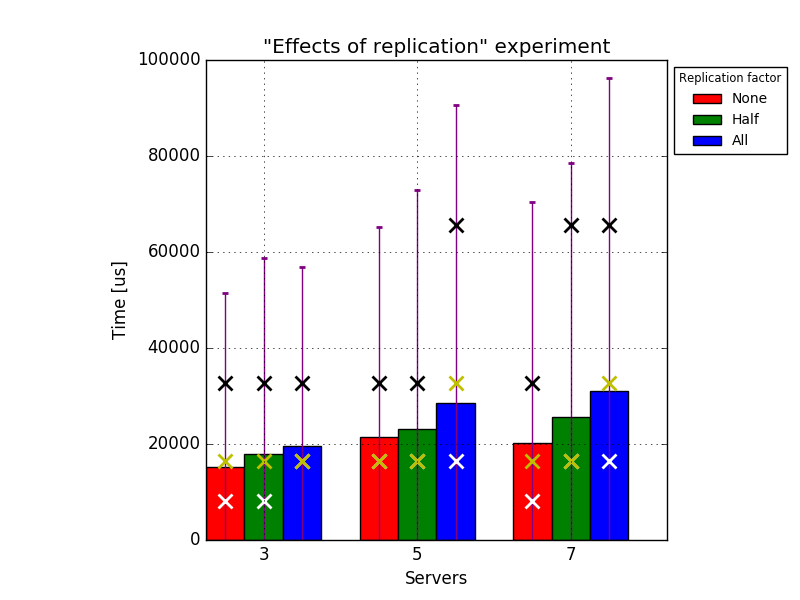
\includegraphics[width=\linewidth]{plots/replication-response_time-set}
	\caption{Response time}
	\label{fig:replication-response-time-set}
\end{subfigure}%
\begin{subfigure}{.5\textwidth}
	\centering
	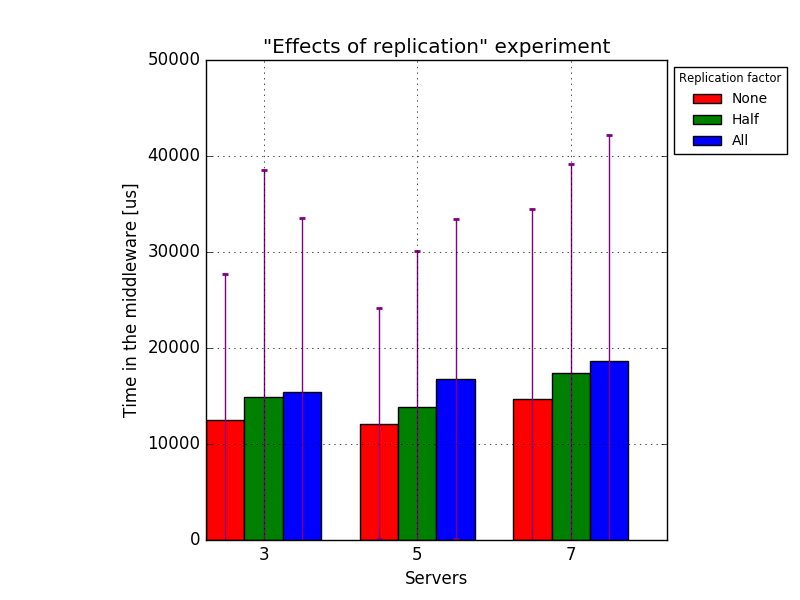
\includegraphics[width=\linewidth]{plots/replication-set}
	\caption{Total time in the middleware}
	\label{fig:replication-set-middleware}
\end{subfigure}

\caption{Measured times for set requests}
\label{fig:replication-set}
\end{figure}

Looking at the figure \ref{fig:replication-set} we can see, that handling incoming requests is no longer the bottleneck of the system for 5 and 7 servers, because increase of the time spent in the middleware results in the corresponding increase in the response time. From this figure we can also see that increasing the replication factor increases noticeably the time spend by the set requests in the middleware and response times for these requets. Setter worker with more servers to replicate to must collect responses from more servers and therefore is more prone to network latencies. More connections are established and if the one response takes longer than usual, it prolongs the total time of the request spent in the middleware.

From the figure \ref{fig:replication-set-servers} we see that it is indeed time spend in the servers that influences the response time significantly. Changing of time in the queue is not relevant here (see figure \ref{fig:replication-set-queue}) - it is similar as we differ the replication factor. 
This can be explained by the way setter workers are implemented in my system (see implementation\footnote{\url{https://gitlab.inf.ethz.ch/matusiaa/asl-fall16-project/blob/master/src/pl/matal/SetterWorker.java}}). When setter worker executes its active waiting loop, it checks whether there are some responses waiting from the server and if yes it handles one of them. After that it checks whether there are any requests from the queue and it yes it handles one of them. This means that every run, if there is a request in the queue, it will be processed. In consequence, increasing replication factor does not affect time spent in the queue significantly - although we have more requests to send, the requests arriving to the queue (which number does not change) can be taken from the queue efficiently.
%although we have only one setter thread, it takes the set request out of the queue quickly, because sending operation is asynchronous. This means, that sending operation itself, as well as collecting responses (using queue-like data structure used in my system and described in the report for milestone 1) is not really time-consuming. With more requests to send we do not notice worse performance of setter worker, since time spent in the queue does not differ significantly as we change the replication factor. We can therefore say that 
With higher replication factor 
%setter worker itself performs similarly, but since 
we, however, have more network requests to send and responses to receive. Therefore we get more time spent in the servers, since we must wait for {\bf all} the responses and therefore we are more prone to network latencies - delay for one response would lead to increasing overall time spent on this operations. 

Figure \ref{fig:replication-set} shows us also that the time spent by set requests in the middleware increases as we increase the number of servers (for replication factor half and all) and varies for replication factor none. This can be explained by both: time spent in the queue and time spent in the servers increasing (for replication factor half and all). With more servers we get more operating system overhead (connected with more threads) and we don't actually have enough cores to run all the threads in parallel at the same time. 

Again, all the data presented in this section comes with high standard deviation. Standard deviation from the response time seems to be more or less proportional to the value itself (see \ref{fig:replication-response-time-set}), but it varies significantly when we look at the detailed times measured by the middleware. This might be because times spent on particular operations in the middleware depend one on another (as analyzed in the section \ref{sec:time-breakdown}) and therefore are prone to more variance. Percentiles presented in the plots seem to be consistent with the average value.

\begin{figure}
\centering
\begin{subfigure}{.5\textwidth}
	\centering
	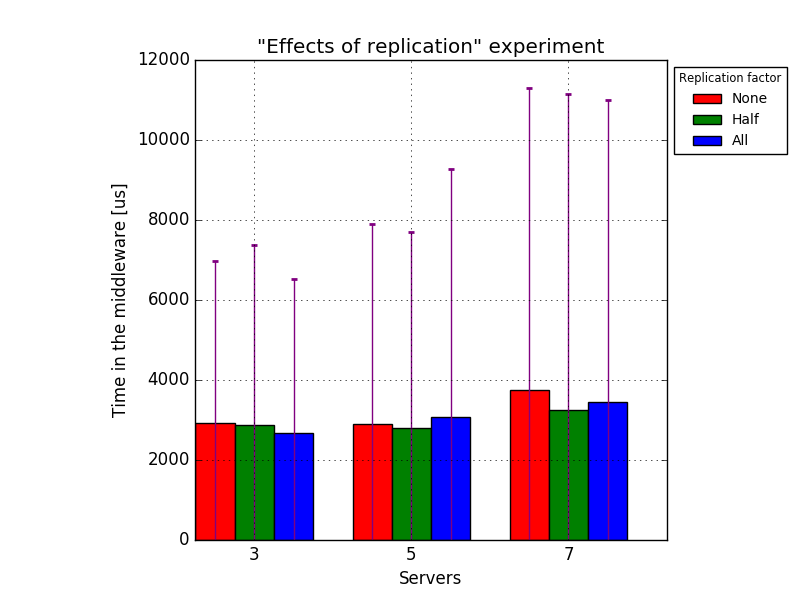
\includegraphics[width=\linewidth]{plots/replication-set-queue}
	\caption{Time in the queue}
	\label{fig:replication-set-queue}
\end{subfigure}%
\begin{subfigure}{.5\textwidth}
	\centering
	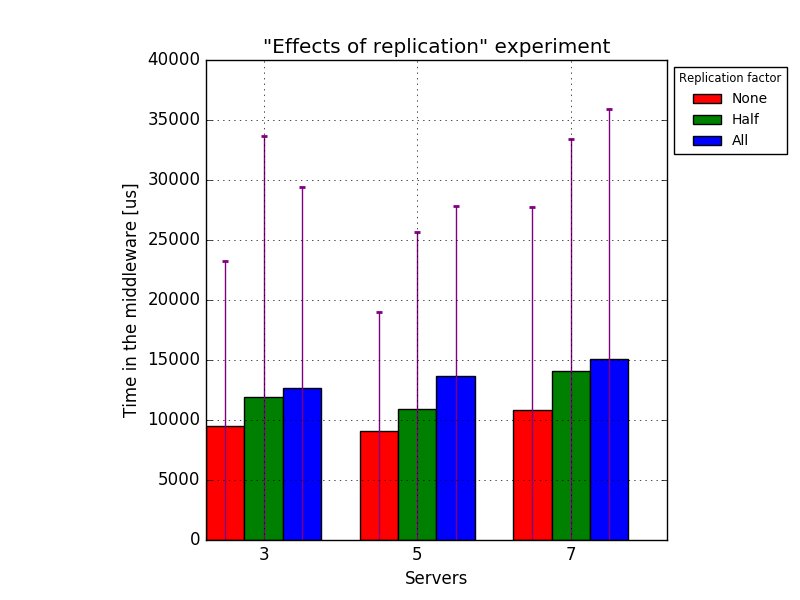
\includegraphics[width=\linewidth]{plots/replication-set-servers}
	\caption{Time in the servers}
	\label{fig:replication-set-servers}
\end{subfigure}
\caption{Breakdown of time spent in the middleware for set requests}
\label{fig:replication-set-breakdown}
\end{figure}

\subsection{Get vs set requests}
\label{sec:replication-get-set}

\begin{figure}
\centering
\begin{subfigure}{.5\textwidth}
	\centering
	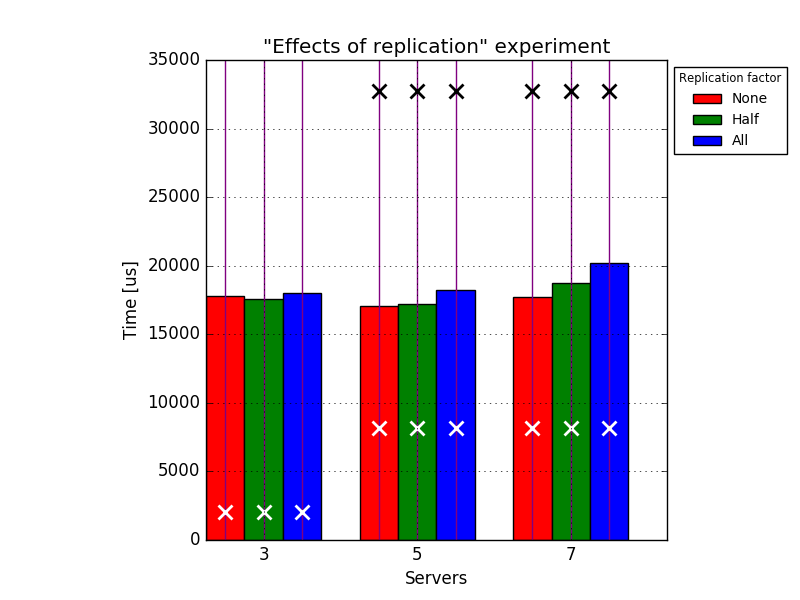
\includegraphics[width=\linewidth]{plots/replication-response_time-get-scaled}
	\caption{Get requests}
\end{subfigure}%
\begin{subfigure}{.5\textwidth}
	\centering
	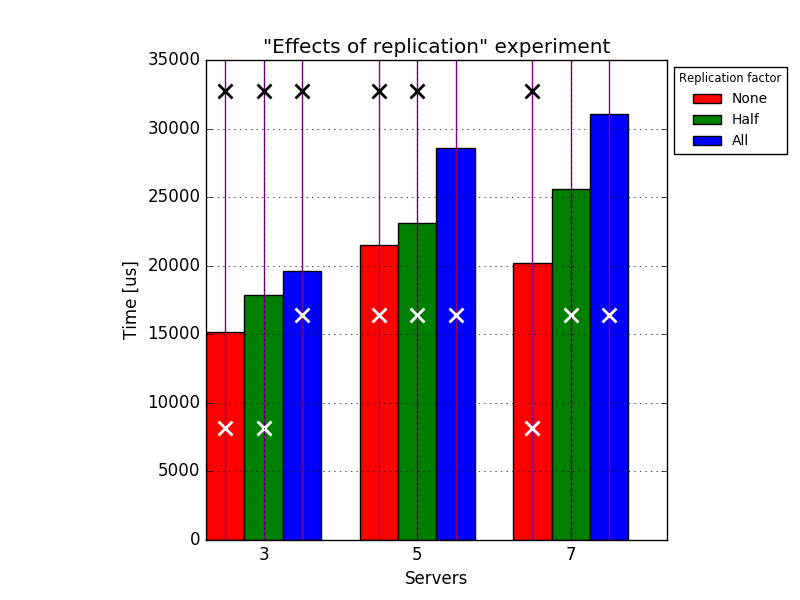
\includegraphics[width=\linewidth]{plots/replication-response_time-set-scaled}
	\caption{Set requests}
\end{subfigure}
\caption{Response times}
\label{fig:replication-response-time-set-get}
\end{figure}

\begin{figure}
\centering
\begin{subfigure}{.5\textwidth}
	\centering
	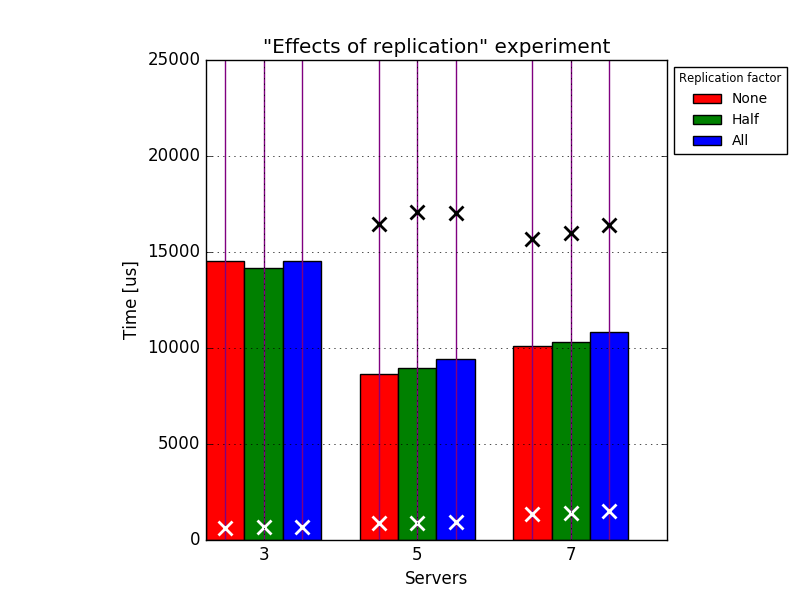
\includegraphics[width=\linewidth]{plots/replication-get-scaled}
	\caption{Get requests}
\end{subfigure}%
\begin{subfigure}{.5\textwidth}
	\centering
	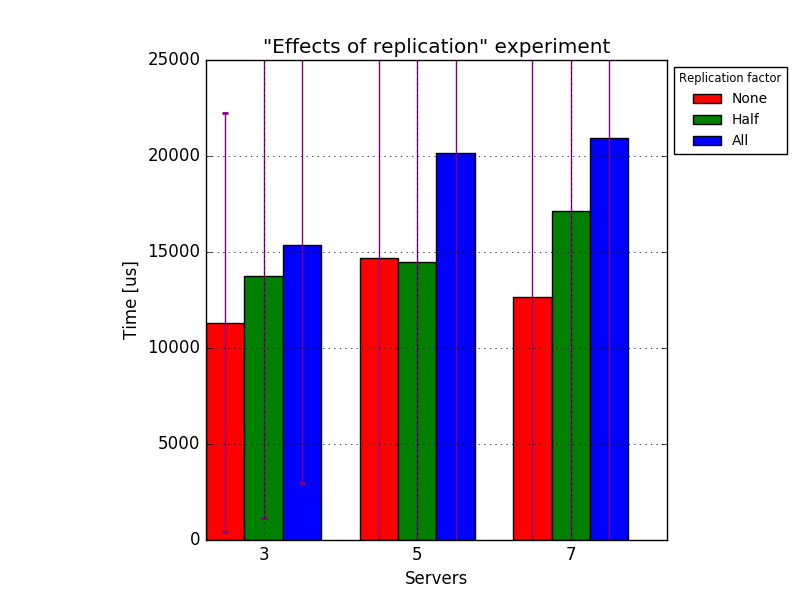
\includegraphics[width=\linewidth]{plots/replication-set-scaled}
	\caption{Set requests}
\end{subfigure}
\caption{Total time spent in the middleware}
\label{fig:replication-set-get}
\end{figure}

Looking at the figures from previous sections as well as the figure
%s \ref{fig:replication-set-get} and 
\ref{fig:replication-response-time-set-get} (plots with the same scale to enable comparison), we can say that usually set requests have higher response time than get requests, especially when we increase the replication factor. This is understandable, since replication affects set requests. However, with no replication and 3 servers we get lower times for set requests. This allows us to say that with no replication and low number of servers synchronous and asynchronous ways of forwarding requests are comparable when it comes to the performance, asynchronous is even a little better. But when we increase number of servers from 3, still with no replication, we notice decrease in performance only for set requests. This is because for set requests the bottleneck is the processing requests already in the middleware, which slows for more servers and therefore increases the response time. 

Looking now at the figure \ref{fig:replication-set-get} we can see, that more scalable method of processing requests inside the middleware (at least for these with no replication) is having many threads synchronously waiting for the response. This is because we chose number of the resources to be optimal for get requests (during first experiment), but have not focused on optimizing time spent by set requests. What is more, design of the middleware does not allow us to tune the performance when it comes to set requests - we can only change resources for processing get requests.  We can tune here this number of threads and to increase the performance also increase the number of cores available. Such tuning and scaling cannot be done, however, for asynchronous processing the requests with one thread (we could though increase number of processing threads, but that was not the point of this method and we do not have enough data to predict behavior of the middleware with this enhancement). This scalability is not, however, visible for clients, because of the bottleneck shifting to accepting incoming requests, as described in previous sections.

Changing of the replication factor seems not to have a significant influence on times connected with get requests (overall time in the middleware, as well as in queue and in servers time). For set requests, however, more time is spent in the servers as we increase the replication factor, which results to higher overall time in the middleware (while time spent in the queue does not change significantly).

The impact of the amount of set requests will be analyzed thoroughly in the section \ref{sec:writes}.

\subsection{Verification of the hypothesis}

My hypothesis was in a large part confirmed by the experimental results. Indeed increasing replication factor influences mostly set requests causing that they stay longer in the middleware. This also affects overall performance and average response time. As we increased of numbers from 3 to 5, the performance indeed increased, and when increasing from 5 to 7 it indeed decreased.

\clearpage

%-----------------------------------------------------------

\section{Effect of Writes}
\label{sec:writes}

\iffalse
In this section, you should study the changes in throughput and response time of your system as the percentage of write operations increases. Use a combination of 3 to 7 servers and vary the number of writes between 1\% and 10\% (e.g. 1\%, 5\% and 10\%). The experiments need to be carried out for the replication factors R=1 and R=all.  

For what number of servers do you see the biggest impact (relative to base case) on performance? Investigate the main reason for the reduced performance and provide a detailed explanation of the behavior of the system. Provide the graphs and tables necessary to support your claims.
\fi

\subsection{Hypothesis}

Increasing number of set requests should decrease the performance of the middleware, especially when we replicate set requests. The necessity to replicate every set request to many servers would cause middleware to be more prone to network latencies (as analyzed in the section \ref{sec:replication}) and having higher percentage of set requests would only intensify this decrease in performance - more percentage of requests will be performed slower. The biggest impact should be visible for 7 servers, since there replicating to all servers will result in having to send set requests to another 6 servers.

\subsection{Experimental setup}

{\small
\smallskip
\begin{tabular}{|c|c|}
\hline Number of servers & 3 - 7 \\ 
\hline Step for number of servers & 2 \\
\hline Number of client machines & 3 \\ 
\hline Virtual clients / machine &  70 \\ 
\hline Threads in the thread pool & 30 \\
\hline Workload & Key 16B, Value 128B, Writes: 1\%, 5\% or 10\% \\
\hline Middleware & Replication: none, all \\ 
\hline Runtime x repetitions & 3 min x 3 \\
\hline Warm-up phase & 1 min \\
\hline Cool-down phase & 1 min \\
\hline Log files & writes\_1, writes\_2, writes\_3, writes\_general, writes\_middleware \\
\hline 
\end{tabular} }
\medskip

For window size I have stayed with 1k, in order to be consistent with the previous experiment (although it shouldn't change the performance)

I have combined the results from 3 repetitions. The variation between repetitions for average was small - values differed from average at most 3,3\%. However the variation for standard deviation was bigger - they differed from average standard deviation at most 17.2\%  This shows that overall variation of data was huge, even between the experiments.

\subsection{Overall performance}

\begin{figure}
\centering
\begin{subfigure}{.5\textwidth}
	\centering
	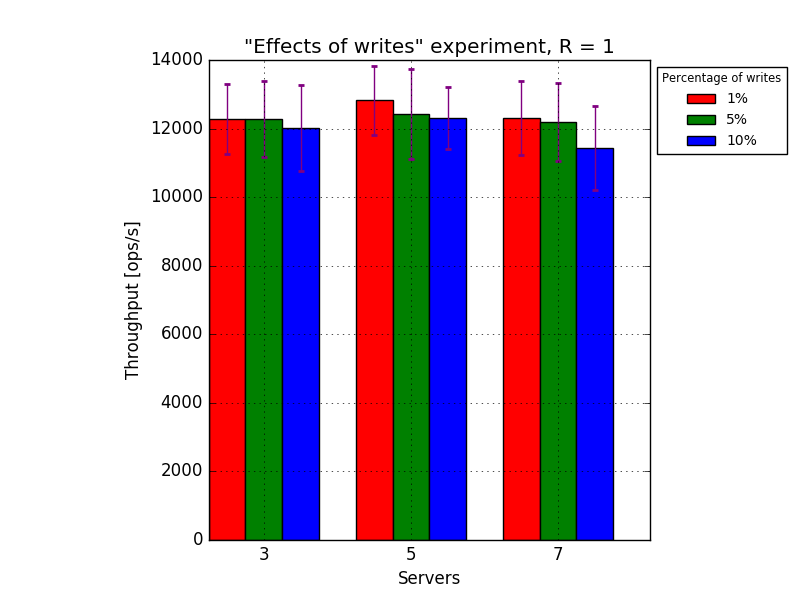
\includegraphics[width=\linewidth]{plots/writes-1-replication}
	\caption{Throughput}
	\label{fig:writes-throughput-1}
\end{subfigure}%
\begin{subfigure}{.5\textwidth}
	\centering
	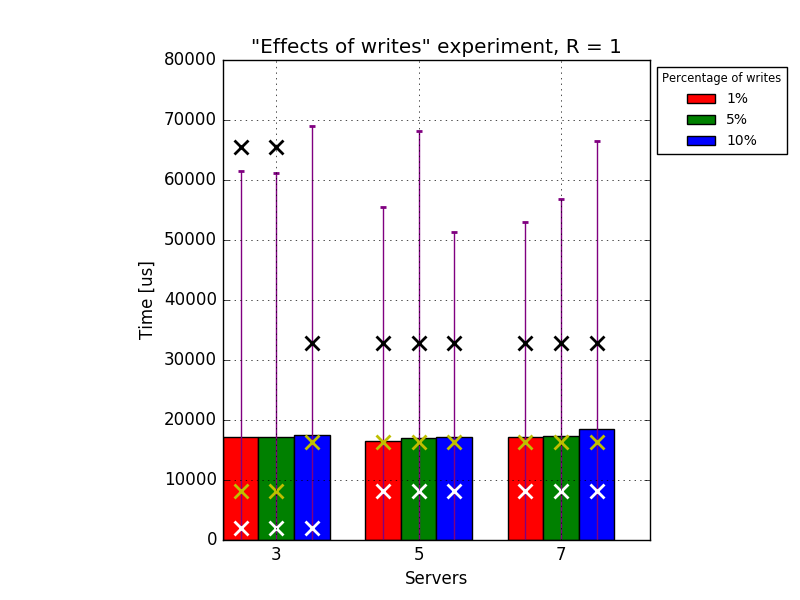
\includegraphics[width=\linewidth]{plots/writes-response_time-1-replication}
	\caption{Response time}
	\label{fig:writes-reponse-time-1}
\end{subfigure}
\caption{Overall performance for the writes experiment with R=1}
\label{fig:writes-overall-none}
\end{figure}

\begin{figure}
\centering
\begin{subfigure}{.5\textwidth}
	\centering
	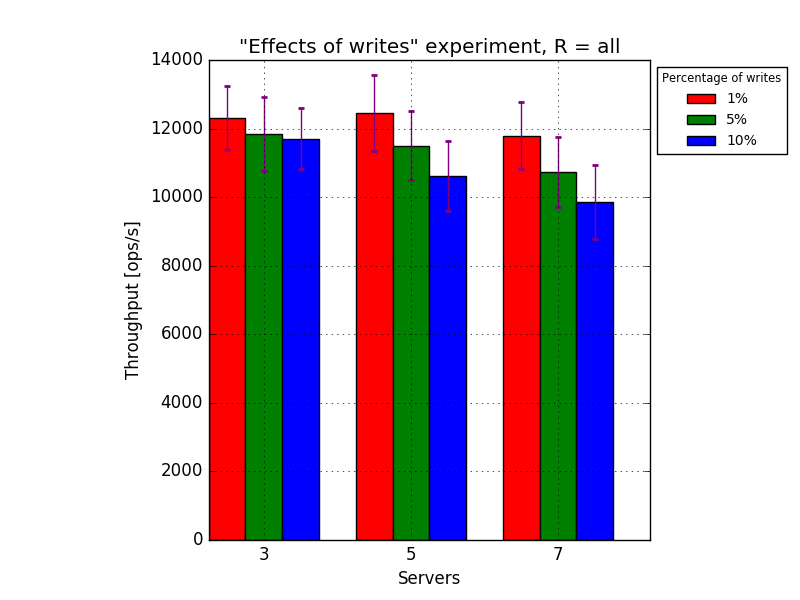
\includegraphics[width=\linewidth]{plots/writes-2-replication}
	\caption{Throughput}
	\label{fig:writes-throughput-2}
\end{subfigure}%
\begin{subfigure}{.5\textwidth}
	\centering
	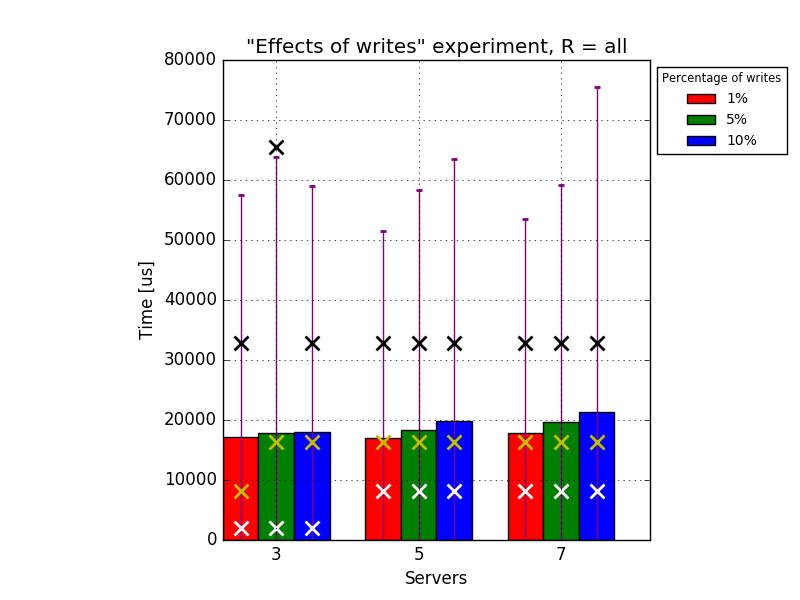
\includegraphics[width=\linewidth]{plots/writes-response_time-2-replication}
	\caption{Response time}
	\label{fig:writes-reponse-time-2}
\end{subfigure}
\caption{Overall performance for the writes experiment with R=all}
\label{fig:writes-overall-all}
\end{figure}

\iffalse
\begin{figure}
\centering
\begin{subfigure}{.5\textwidth}
	\centering
	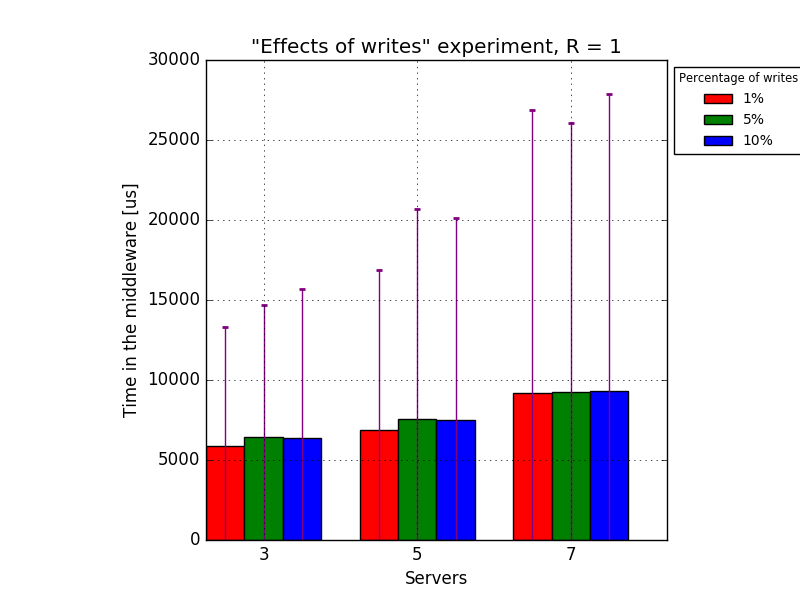
\includegraphics[width=\linewidth]{plots/writes-all-1-replication}
	\caption{Replication factor = 1}
	\label{fig:writes-all-1}
\end{subfigure}%
\begin{subfigure}{.5\textwidth}
	\centering
	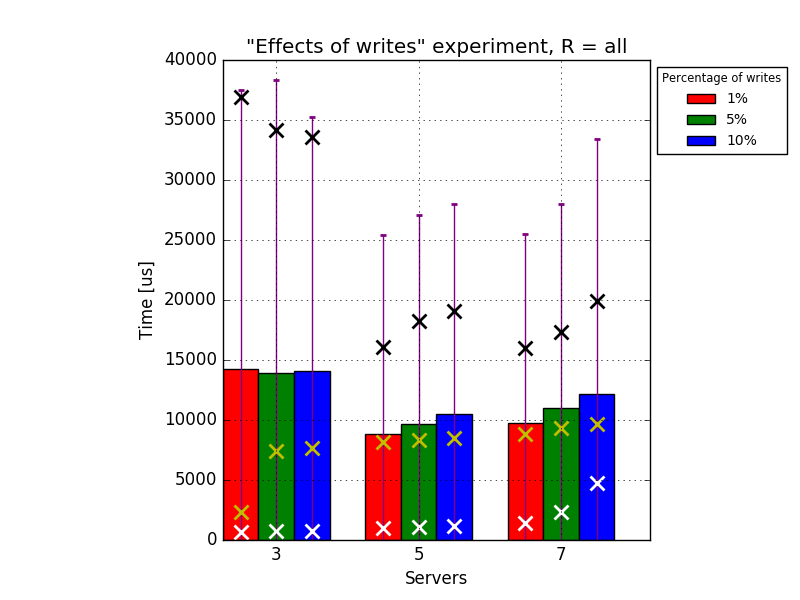
\includegraphics[width=\linewidth]{plots/writes-all-2-replication}
	\caption{Replication factor = all}
	\label{fig:writes-all-2}
\end{subfigure}
\caption{Total time spent in the middleware}
\label{fig:writes-all}
\end{figure}
\fi

As we can see from figure \ref{fig:writes-overall-none} and \ref{fig:writes-overall-all} significant impact of changing writes percentage is only visible for the replication factor equals to all. This is because with no replication processing set requests takes approximately the same time as get requests so changing write percentage will not affect the performance. Although worker threads present different approach for processing requests for get and set requests, we could see in previous experiments that it is time spent in the servers that is most significant and time spent being processed by the worker threads is not that important. Therefore, since for no replication we have the same number of requests to servers per request in the middleware (equals to 1), we do not notice difference in the response time for these types of threads, so changing their ratio does not influence the overall performance significantly. We notice, however, slight decrease in performance for more servers, because, as we could see from section \ref{sec:replication-get-set}, for bigger number of servers set requests are taking a little longer to process than get requests. 

For replication to all servers, however, we can see a significant decrease in the performance as we increase the writes percentage. This is because set requests now need more time to be processed by the middleware (see section \ref{sec:replication-get-set}) than get requests. Therefore, as we increase the percentage of set requests, we increase overall response time, which means decrease in the performance.

To find out for what numbers of servers there is the highest impact on changing the writes percentage we can use a table presented below, where we can see the throughput for different configurations with replication factor equals to all. As base case we take the throughput for 3 servers, 1\% write requests and no replication - the throughput for this configuration equals to 12285 [ops/s].
\medskip

{\small
\begin{tabular}{|c|c|c|c|c|}
\hline \bf{Servers} & \parbox[t]{2.7cm}{\bf{Throughput for \\1\% writes [ops/s]}} & \parbox[t]{2.7cm}{\bf{Throughput for\\ 10\% writes [ops/s]}} & \parbox[t]{3.2cm}{\bf{Ratio (10\% writes \\to 1\% writes)}} & \parbox[t]{3.2cm}{\bf{Ratio (10\% writes \\to the base case)}} \\[3ex] 
\hline 3 & 12315 & 11791 & 0.96 & 0.96 \\ 
\hline 5 & 12447 &  10615 & 0.85 & 0.86 \\
\hline 7 & 11791 & 9858 & 0.83 & 0.80 \\
\hline 
\end{tabular}}
\medskip

We can see that the impact of increasing the percentage of writes (from 1\% to 10\%) is increasing as we increase the number of servers. This is because when we replicate to all servers, with more servers we have to send more requests. This means that with more servers we notice the most impact on the response time of set requests and set requests are being processed longer comparing to get requests. As we increase percentage of writes, this impact becomes intensified, since requests that need more time to be processed (set requests) are now more often. Consequently, the most impact relative to the base case is for higher number of servers (7) and writes percentage 10\%, which is connected with impact of increasing writes percentage as well as increasing servers number - for 7 servers we have the lowest throughput with 1\% writes.

\subsection{Get requests}

\begin{figure}
\centering
\begin{subfigure}{.5\textwidth}
	\centering
	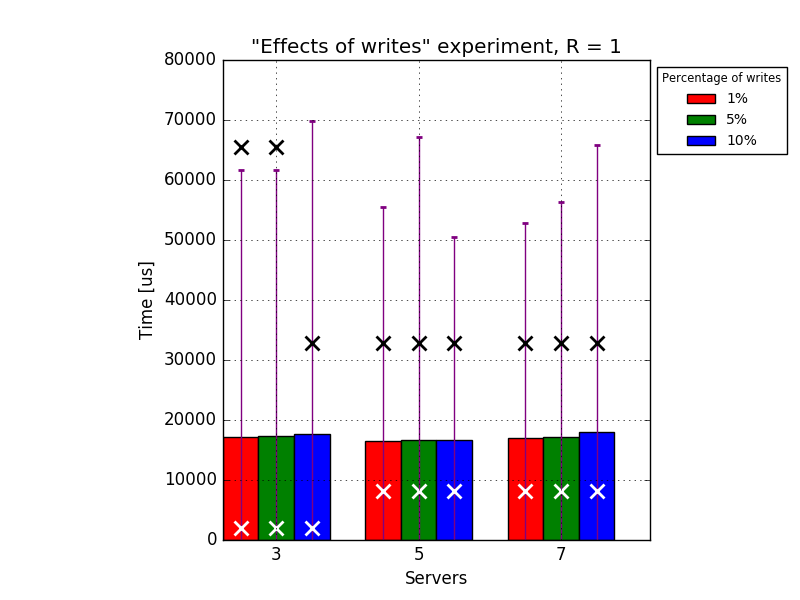
\includegraphics[width=\linewidth]{plots/writes-response_time-get-1-replication}
	\caption{Replication factor = 1}
	\label{fig:writes-get-1}
\end{subfigure}%
\begin{subfigure}{.5\textwidth}
	\centering
	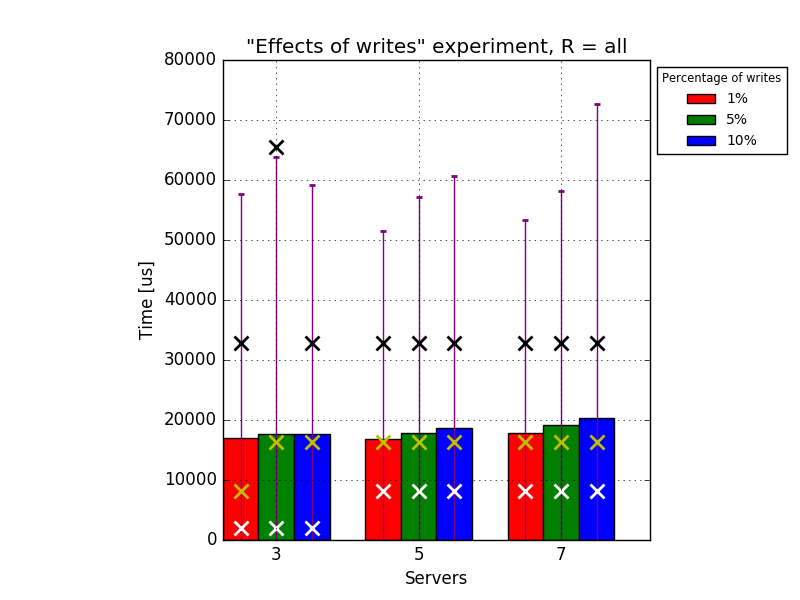
\includegraphics[width=\linewidth]{plots/writes-response_time-get-2-replication}
	\caption{Replication factor = all}
	\label{fig:writes-get-2}
\end{subfigure}
\caption{Response time for get requests}
\label{fig:writes-response-time-get}
\end{figure}

\begin{figure}
\centering
\begin{subfigure}{.5\textwidth}
	\centering
	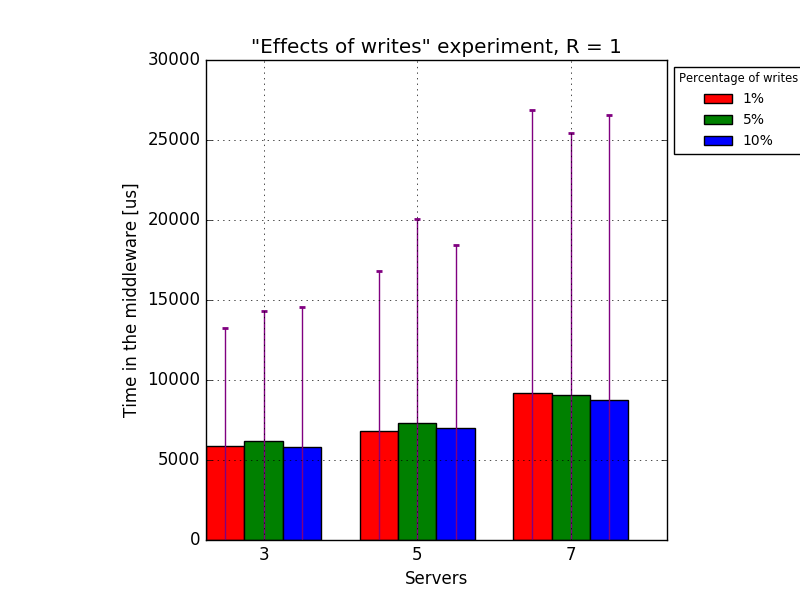
\includegraphics[width=\linewidth]{plots/writes-get-1-replication}
	\caption{Replication factor = 1}
	\label{fig:writes-get-1}
\end{subfigure}%
\begin{subfigure}{.5\textwidth}
	\centering
	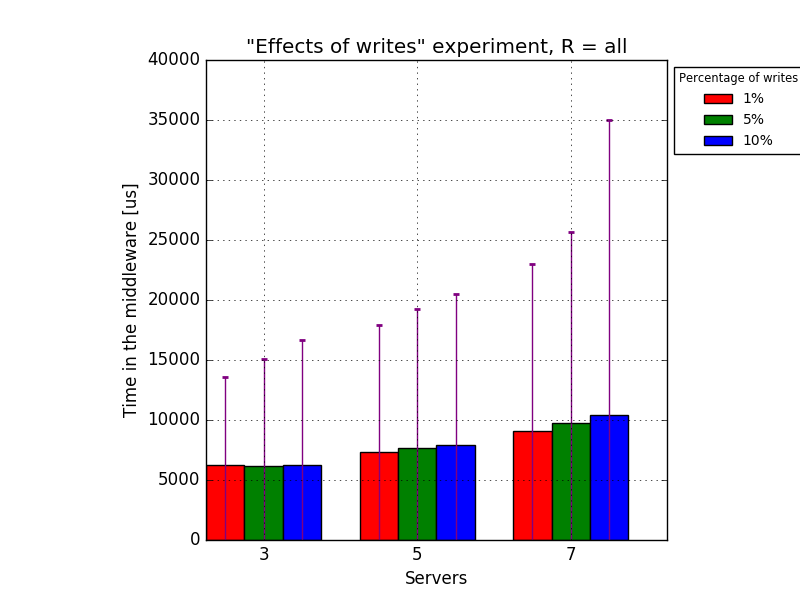
\includegraphics[width=\linewidth]{plots/writes-get-2-replication}
	\caption{Replication factor = all}
	\label{fig:writes-get-2}
\end{subfigure}
\caption{Total time spent in the middleware for get requests}
\label{fig:writes-get}
\end{figure}

As we can see from figure \ref{fig:writes-response-time-get} and \ref{fig:writes-get} get requests are not significantly affected by changing the percentage of set requests (for both replication factors). This is because percentage of get requests does not change very much (it varies: 99\%, 95\% and 90\%), so the load for getter workers is similar. What is more we have chosen optimal number of threads which handle get requests with precision 10, so changing amount of get requests slightly (at most 10\%) does not affect the performance much. We can even see a slight decrease in the performance, as we increase replication factor, which might be cause by more work that setter threads has to do, which causes getter threads to get less operating system resources. 

Impact of changing the number of servers for get requests has been thoroughly analyzed in the section \ref{sec:replication-get}. Again, we can see that for 5 and 7 servers the bottleneck is handling new requests.

\subsection{Set requests}

\begin{figure}
\centering
\begin{subfigure}{.5\textwidth}
	\centering
	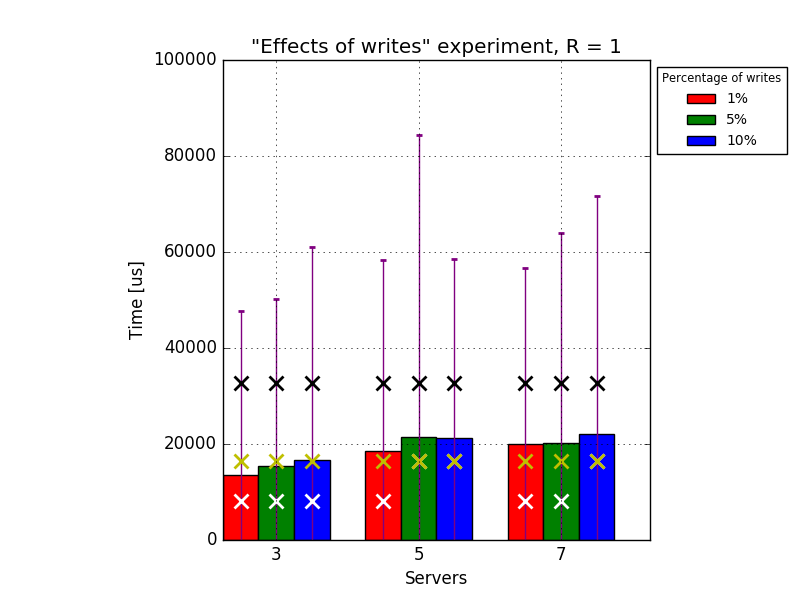
\includegraphics[width=\linewidth]{plots/writes-response_time-set-1-replication}
	\caption{Replication factor = 1}
	\label{fig:writes-set-1}
\end{subfigure}%
\begin{subfigure}{.5\textwidth}
	\centering
	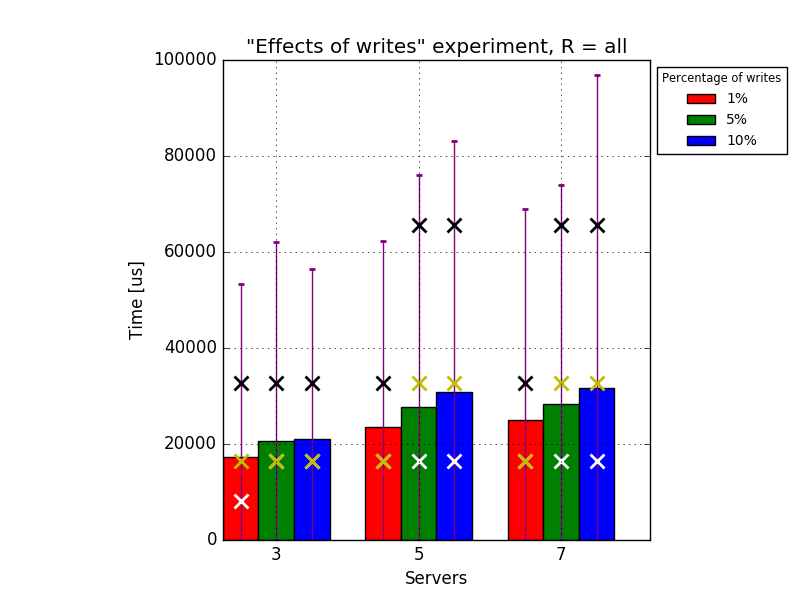
\includegraphics[width=\linewidth]{plots/writes-response_time-set-2-replication}
	\caption{Replication factor = all}
	\label{fig:writes-set-2}
\end{subfigure}
\caption{Response time for set requests}
\label{fig:writes-response-time-set}
\end{figure}


\begin{figure}
\centering
\begin{subfigure}{.5\textwidth}
	\centering
	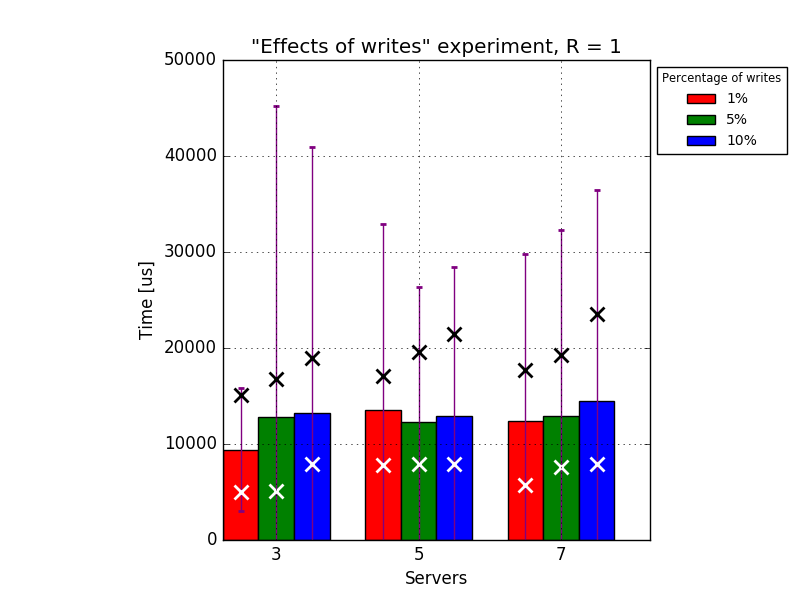
\includegraphics[width=\linewidth]{plots/writes-set-1-replication}
	\caption{Replication factor = 1}
	\label{fig:writes-set-1}
\end{subfigure}%
\begin{subfigure}{.5\textwidth}
	\centering
	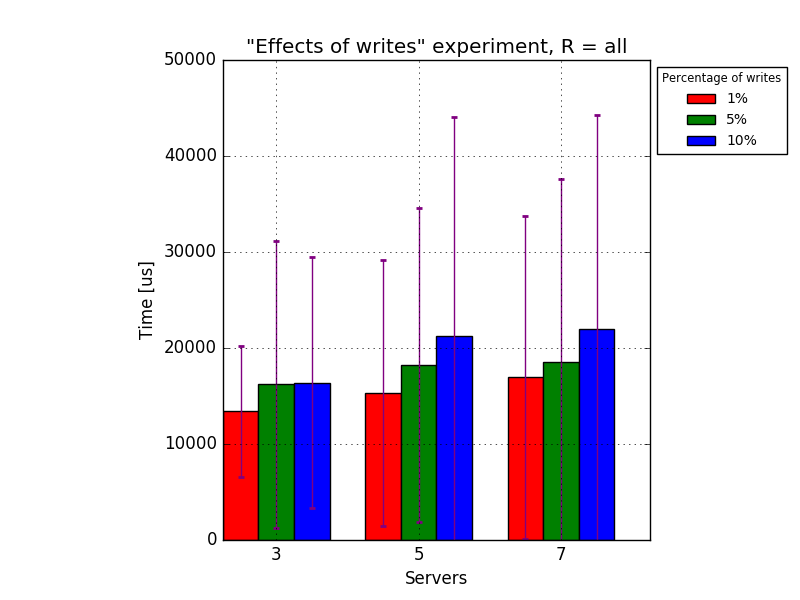
\includegraphics[width=\linewidth]{plots/writes-set-2-replication}
	\caption{Replication factor = all}
	\label{fig:writes-set-2}
\end{subfigure}
\caption{Total time spent in the middleware for set requests}
\label{fig:writes-set}
\end{figure}

The situation looks differently for set requests. We can see from figure \ref{fig:writes-response-time-set} and  \ref{fig:writes-set} that for no replication changes in percentage of writes do not influence significantly time spent in the middleware and response time for set requests (apart from 3 servers, where increase from 1\% to 5\% can be considered significant). For replication factor equals to all we can see, however, a significant increase in the time spent in the middleware and response time for set requests, especially for 5 and 7 servers. When we look at the figure \ref{fig:writes-set-breakdown-2} we can see that this is caused by the increase of the time spent in the servers, because time spent in the queue does not change noticeable when we vary writes percentage. Although we do increase the number of set requests, we still can take requests from the queue efficiently - like described in the section \ref{sec:replication-set}
%
%This can be explained by the way setter workers are implemented in my system (see implementation\footnote{\url{https://gitlab.inf.ethz.ch/matusiaa/asl-fall16-project/blob/master/src/pl/matal/SetterWorker.java}}). When setter worker executes its active waiting loop, it checks whether there are some responses waiting from the server and if yes it handles one of them. After that it checks whether there are any requests from the queue and it yes it handles one of them. This means that every run, if there is a request in the queue, it will be processed. In consequence, increasing writes percentage does not affect time spent in the queue significantly - although we have more requests, they can be taken from the queue effectively. 
However, as we increase the percentage of writes with replication to all servers we also increase the number of responses that have to be processed. Because we replicate to all servers this results in an increased time spent in the servers. Let's remember here that time spent in the servers consists also of waiting of responses in the middleware to be process by the setter thread. This means that with increasing percentage of writes more responses have to be processed by the middleware and sometimes they will have to wait to be processed by the middleware because setter thread will be busy. 

To sum up this analysis, as we increase the percentage of writes, number of requests in the queue and number of requests send to server increase by the same factor, but increase in the time is more visible for requests send to server, since we replicate each of them (with more requests decrease in the performance is more visible). The possible area of improvement here might be to vary the proportion of handling requests from the queue and responses from the server. If we e.g. for every processed request taken from the queue we process 2 responses from the servers (if available), then for replication factor equal to all the performance might improve.

Impact of changing the number of servers for get requests has been thoroughly analyzed in the section \ref{sec:replication-set}.

\begin{figure}
\centering
\begin{subfigure}{.5\textwidth}
	\centering
	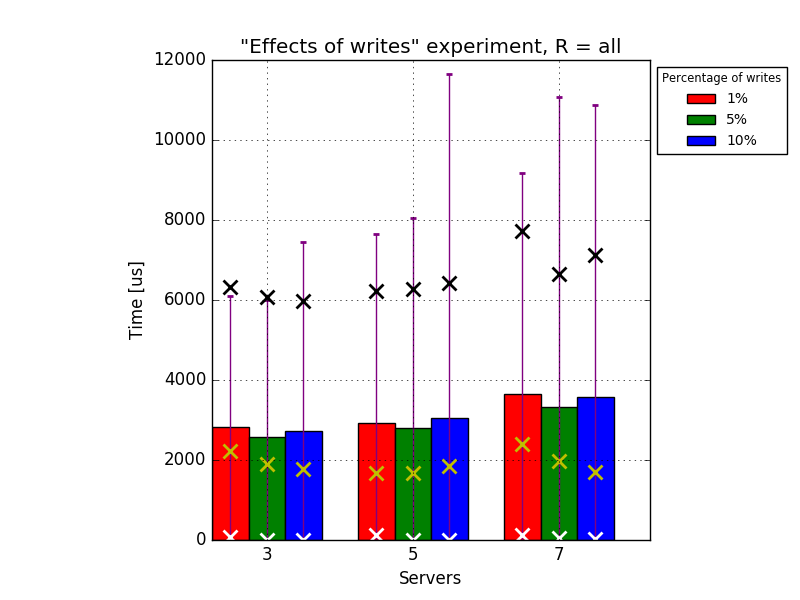
\includegraphics[width=\linewidth]{plots/writes-set-queue-2-replication}
	\caption{Time spent in the queue}
	\label{fig:writes-set-queue-2}
\end{subfigure}%
\begin{subfigure}{.5\textwidth}
	\centering
	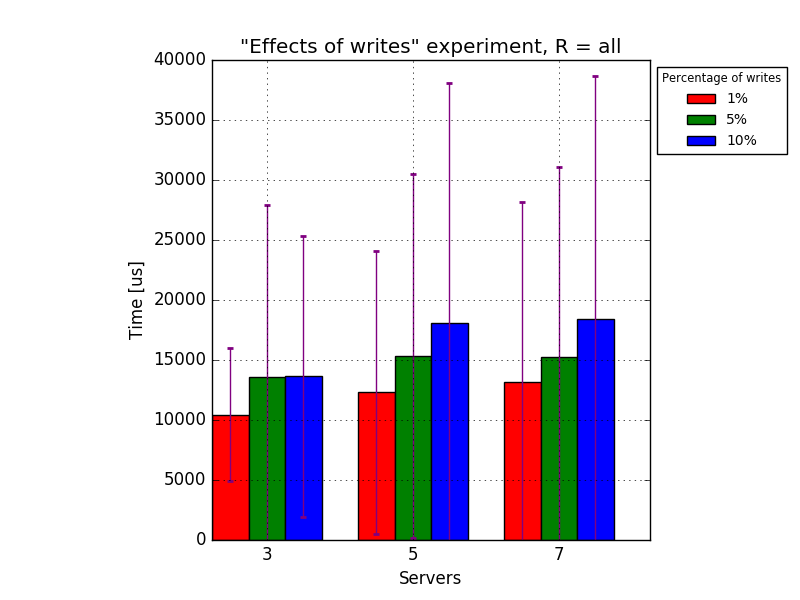
\includegraphics[width=\linewidth]{plots/writes-set-servers-2-replication}
	\caption{Time spent in the servers}
	\label{fig:writes-set-servers-2}
\end{subfigure}
\caption{Breakdown of time spent in the middleware for set requests (replication factor = all)}
\label{fig:writes-set-breakdown-2}
\end{figure}

\subsection{Verification of hypothesis}
As predicted, increasing the writes percentage resulted in the performance decreasing, especially for replicating to all servers. This can be explained by higher number of set requests, which are processed slower, as well as increase in the time set requests are processed when there are more of them. 


\clearpage

\section*{Logfile listing}

\begin{tabular}{|c|p{12.0cm}|}
\hline \textbf{Short name }& \textbf{Location} \\ 
\hline  overall\_1 & \url{https://gitlab.inf.ethz.ch/matusiaa/asl-fall16-project/blob/master/logs/milestone2/overall_1.tar.gz}\\ 
\hline overall\_2 & \url{https://gitlab.inf.ethz.ch/matusiaa/asl-fall16-project/blob/master/logs/milestone2/overall_2.tar.gz}\\ 
\hline overall\_3 & \url{https://gitlab.inf.ethz.ch/matusiaa/asl-fall16-project/blob/master/logs/milestone2/overall_3.tar.gz}\\ 
\hline overall\_4 & \url{https://gitlab.inf.ethz.ch/matusiaa/asl-fall16-project/blob/master/logs/milestone2/overall_4.tar.gz}\\ 
\hline overall\_5 & \url{https://gitlab.inf.ethz.ch/matusiaa/asl-fall16-project/blob/master/logs/milestone2/overall_5.tar.gz}\\ 
\hline overall\_general & \url{https://gitlab.inf.ethz.ch/matusiaa/asl-fall16-project/blob/master/logs/milestone2/overall_general.tar.gz}\\ 
\hline  detailed\_1 & \url{https://gitlab.inf.ethz.ch/matusiaa/asl-fall16-project/blob/master/logs/milestone2/detailed_1.tar.gz}\\
\hline  detailed\_2 & \url{https://gitlab.inf.ethz.ch/matusiaa/asl-fall16-project/blob/master/logs/milestone2/detailed_2.tar.gz}\\ 
\hline  detailed\_3 & \url{https://gitlab.inf.ethz.ch/matusiaa/asl-fall16-project/blob/master/logs/milestone2/detailed_3.tar.gz}\\ 
\hline  detailed\_4 & \url{https://gitlab.inf.ethz.ch/matusiaa/asl-fall16-project/blob/master/logs/milestone2/detailed_4.tar.gz}\\ 
\hline  detailed\_5 & \url{https://gitlab.inf.ethz.ch/matusiaa/asl-fall16-project/blob/master/logs/milestone2/detailed_5.tar.gz}\\ 
\hline  detailed\_general & \url{https://gitlab.inf.ethz.ch/matusiaa/asl-fall16-project/blob/master/logs/milestone2/detailed_general.tar.gz}\\ 
\hline  max\_throughput\_detailed & \url{https://gitlab.inf.ethz.ch/matusiaa/asl-fall16-project/blob/master/logs/milestone2/max_throughput_detailed.tar.gz}\\ 
\hline  replication\_1 & \url{https://gitlab.inf.ethz.ch/matusiaa/asl-fall16-project/blob/master/logs/milestone2/replication_1.tar.gz}\\ 
\hline  replication\_2 & \url{https://gitlab.inf.ethz.ch/matusiaa/asl-fall16-project/blob/master/logs/milestone2/replication_2.tar.gz}\\ 
\hline  replication\_3 & \url{https://gitlab.inf.ethz.ch/matusiaa/asl-fall16-project/blob/master/logs/milestone2/replication_3.tar.gz}\\ 
\hline  replication\_general & \url{https://gitlab.inf.ethz.ch/matusiaa/asl-fall16-project/blob/master/logs/milestone2/replication_general.tar.gz}\\ 
\hline  replication\_middleware & \url{https://gitlab.inf.ethz.ch/matusiaa/asl-fall16-project/blob/master/logs/milestone2/replication_middleware.tar.gz}\\ 
\hline  writes\_1 & \url{https://gitlab.inf.ethz.ch/matusiaa/asl-fall16-project/blob/master/logs/milestone2/writes_1.tar.gz}\\ 
\hline  writes\_2 & \url{https://gitlab.inf.ethz.ch/matusiaa/asl-fall16-project/blob/master/logs/milestone2/writes_2.tar.gz}\\ 
\hline  writes\_3 & \url{https://gitlab.inf.ethz.ch/matusiaa/asl-fall16-project/blob/master/logs/milestone2/writes_3.tar.gz}\\ 
\hline  writes\_general & \url{https://gitlab.inf.ethz.ch/matusiaa/asl-fall16-project/blob/master/logs/milestone2/writes_general.tar.gz}\\ 
\hline  writes\_middleware & \url{https://gitlab.inf.ethz.ch/matusiaa/asl-fall16-project/blob/master/logs/milestone2/writes_middleware.tar.gz}\\ 
\hline 
\end{tabular}

\pagebreak

\section*{Appendix - changes in the source code}

In order to enable distinction between set and get requests in the middleware logs, I have added to my implementation writing the type of request for every log entry\footnote{\url{https://gitlab.inf.ethz.ch/matusiaa/asl-fall16-project/blob/master/src/pl/matal/Request.java}:59-63}. What is more, with higher number of clients, my middleware was sometimes not forwarding received requests and responses correctly. This was due to not checking for emptiness of the buffer after sending the first part of the message - sending should be continued till the buffer is empty. This bug was fixed in the source code\footnote{\url{https://gitlab.inf.ethz.ch/matusiaa/asl-fall16-project/blob/master/src/pl/matal/SetterWorker.java}:98-100} and corrected code was used for running the experiments for this milestone. Fixing this bug should not correspond to changes in performance comparing with the stability experiment - in that experiment I didn't notice any problems and simply checking for the buffer emptiness does not influence overall system design and the performance.
 
\end{document}